 \documentclass{article}
\usepackage[utf8]{inputenc}




\usepackage{geometry}                		
\geometry {letterpaper, left=2.5 cm, right=2.5 cm, top=2.5cm, bottom=2.5 cm}    


\usepackage{multirow}
\usepackage{graphicx}		
\graphicspath{ {c:} }
\usepackage{setspace}
\usepackage[version=4]{mhchem}
\doublespace
\usepackage{siunitx}
\usepackage{natbib}
\usepackage{amsmath}
\usepackage{bm}
\usepackage{amsfonts}
\usepackage{lineno}
\usepackage[sharp]{easylist}%makes nice outlines.  Use # for symbol
\usepackage{blkarray}
\begin{document}
%\maketitle

{\Large \noindent \bf %Approaches for handling missing data in ecological time series
Accounting for missing data in autoregressive models of ecological time series
}

\medskip

% Author list TBD, this list based on Amy's ESA abstract
\noindent Alice Stears, Melissa DeSiervo, Dusty Gannon, Alice Carter, Christa L. Torrens, Amy Patterson, Topher Weiss-Lehman, Saheed Olaide Jimoh, Courtenay Ray, Joanna Blaszczak, Josh Jahner, Lauren Shoemaker


\clearpage

\begin{linenumbers}

\section*{Abstract (200 words max)} % From Amy's ESA abstract
Long term time series are extremely valuable and increasingly available tools for understanding ecological systems. Unfortunately, missing data can threaten the utility of long time series. While several methods exist, there is no established best practice for handling missing data in time series. Using real and simulated data from primary productivity in a river and population counts of great tits (\textit{Parus major}), we explore the performance of six missing data methods across several missing data scenarios that vary the amount and distribution of missing data. We evaluated method performance using bias, average absolute error, prediction error, and coverage of the confidence interval, and we found that performance depended on the type of data available. Overall, missing data were most likely to affect estimates of autoregressive parameters and population growth variables where current population is a direct function of past population. When data were missing at random, regression coefficient estimates were predicted well regardless of missing data. For the simulated river data, data augmentation and the Kalman filter performed well, while multiple imputation, simple data deletion, and complete case data deletion resulted in biased estimates and poor accuracy of autoregressive parameters. In addition to their poor average performance, the inferior methods also overestimated their own accuracy, with multiple imputation in particular outputting 95\% confidence intervals that included the true autoregression values only 40\% of the time when half of the data were missing. When data were missing not at random, all the methods performed quite poorly for high amounts of missing data. For the simulated population data, the best performing methods were data augmentation and complete case data deletion, while simple data deletion was by far the worst performing method. Surprisingly, the analyses using the real river data and the great tit data did not always follow the same trends as the simulated data. For the river data, projections relied mostly on covariate predictors rather than autoregressive effects, showing that most methods work well with high quality predictors. For the population data, missing covariates and unexplained variation in real data reduced performance differences between methods and led to high variance in predictive ability. We recommend that practitioners use the Kalman filter and data augmentation for missing data with Gaussian error, while using extreme caution for any data that are missing not at random. Practitioners should also avoid using simple data deletion wherever possible, especially for population data.

\section*{Introduction} 

%%OUTLINE OF THE INTRODUCTION%%

% New Version (October 2024--feel free to comment!)
% I. Start with there's been a push to collect long term data in ecology, simultaneously with a recent push for rediscovering/analyzing historic datasets (e.g. cherry blossom data). For both scenarios, missingness is common and presents a huge challenge, limiting analyses of large, robust datasets that have been huge efforts to collect.
    % 1. Ecological data collection is particularly prone to missingess because of environmental stochasticity, difficult access, etc.
    % 2. Time series are also more likely to have missingness we can't deal by simply collecting more data, since we can't backfill data at points in time that have already passed. 
 
% II. Missing data in ecological settings can present unique challenges.
    % 1. Ecological data are often structured as autoregressive time series in which current data partially depend on the value of previous data. In such settings, missing values can be especially problematic as they affect inference on multiple data points.
    % 2. Additionally, ecological data can often correspond to non-normal distributions (e.g., count data) that have not been rigorously explored with existing methods of dealing with missing data.
    %3. (very general) There are different types of missigness that can occur in ecological time series (give examples that illustrate the main types of missingess that we include in this MS -- MAR and MCAR w/ different levels of autocorrelation).  
% III. Methods have been proposed for dealing with missing data. However, many were formulated without considering the challenges of missing data in autoregressive time series. While there are some methods that have been developed specifically to address missingness in autoregressive time series, we do not have clear information about how these various methods perform with different types and amounts of missingness and with different types of time series data. 
% IV. Here, we evaluate the precision and accuracy of different statistical approaches for dealing with missing data in autoregressive models of ecological time series data. We test these missing data approaches on real and simulated datasets with both Gaussian and Poisson error distributions. We artificially introduce missingness of different types and increasing amounts into all of these time series, and quantify the performance of different missing data approaches across these three axes of variation in the time series data used (error distribution of the time series, amount of missingness, and type of missingness). This comparison of approaches for dealing with missing data in ecological time series provides a novel comparison of multiple previously-proposed methods of dealing with missing data, some of which have not been previously used with time series data, and will help ecologists determine which method is best suited for addressing the problem of missing data in their particular time series dataset. 

%------------------------------------------


Long-term ecological time series contribute to our understanding of many ecological phenomena, from the impacts of species diversity on predator-prey dynamics to patterns of nutrient cycling in ecosystems \citep{Hughes2017, Likens1970, Sinclair2003}. There has been a concerted effort in recent years to facilitate the collection of long-term ecological datasets (e.g. the U.S National Science Foundation Long Term Ecological Research Program (NSF LTER), and the Smithsonian Forest Global Earth Observatory (ForestGEO)), as well as to re-analyze historical long-term datasets with modern methods \citep{Adler2009, Buma2017}. Long-term time series of ecological data, as well as ecological time series in general, are likely to have missing observations, due largely to unpredictable environmental barriers to complete data collection that are difficult if not impossible to overcome \citep{lopucki2022handling, nakagawa_missing_2008}. These include incomplete data collection due to faulty sensors \citep{hossie_confronting_2021}, inaccessibility of field sites due to weather or even a global pandemic, as well as human error during the data entry or collection processes that necessitates removing observations due to inaccuracy. Due to the temporal nature of time series data, it is impossible to retroactively collect data to fill in missing observations. These missing data have cascading negative effects on subsequent analysis including reduced statistical power \citep{kang2013prevention, moritz_imputets_2017} and biased estimation of parameters, leading to both inaccurate and imprecise conclusions \citep{aleryani2018dealing, kim_transcending_2018, junger_imputation_2015}

The prevalence of missing data in ecological time series data is itself problematic, but can be compounded by the characteristics of ecological time series and the statistical approaches used to model them. First, ecological data are often structured as autoregressive time series in which a current data point partially depends on the value of previous data (e.g., population counts through time or nutrient fluxes within a system).  This means that each observation is both a response to past observations and a predictor for subsequent observations, so a single missing observation could lead to the deletion of multiple data points. As such, seemingly low rates of missing data in autoregressive time series can have strong negative affects on the precision and bias of statistical inference. Further, autoregressive time series with non-Gaussian error distributions are common in ecology, which can add to the challenge of building statistical models and dealing with missing values in these datasets. For example, population count data may be modeled using a Poisson or negative binomial distribution, which precludes the use of classical ARIMA models. Approaches that impute missing values or use model-based approaches that estimate missing values as model parameters must be adjusted to account for time series with non-Gaussian error distributions. In addition to accounting for the characteristics of the time series as a whole, one must also account for the missing data mechanism, i.e. the statistical relationship between observations and the probability of missing data. Missing data points can be Missing Completely at Random (MCAR), Missing at Random (MAR), or Missing Not at Random (MNAR) \citep[][Fig. \ref{fig:missingtypes}]{rubin_inference_1976, nakagawa_missing_2015}. Data are MCAR when the probability of missing data in the response variable is independent of the values of both the missing and present observations in the response and predictor variables \citep{nakagawa_missing_2015, horton2007much}. When data are MCAR, the pattern of missingness can vary along a spectrum from low autocorrelation (whether a previous data point is missing does not impact whether the current data point is missing) to high autocorrelation (if the previous data point is missing, the current data point is more likely to be missing). Data are MNAR when the probability of missingness in the response variable depends on missing values in either the predictor or response variables: that is, it depends on either the value of the missing data point itself (e.g. a temperature sensor can't record values above a threshold, so observations above that value are missing), or on missing observations in a predictor variable (e.g.  high streamflows may create missing or NA data in both the stream gage and turbidity sensors, so the missing turbidity values are dependent on the missing stream gage values). Data are MAR when missing data points are associated with observed values of another variable or  variables and are independent of any unobserved or missing variables (e.g. apopulation age-weight dataset is  missing weights for  young-of-the-year because that age class is considered  too delicate to handle )  \citep{newman_missing_2014, ellington_using_2015, nakagawa_missing_2015}. The key difference between MAR and MNAR data is whether the observations that affect missingness are observed (and can thus be controlled for), which describes MAR data, or unobserved, which describes MNAR data (\citep{nakagawa_model_2011}. In addition, once you control for the known effects in MAR data, it can be handled like MCAR, or missing completely at random data (\citep{nakagawa_missing_2015}.  [and others]

Our analyses focus on MAR and MNAR only because they are prevalent in ecological time series, and are concerned only with missing values in the response variable, which makes it easier to compare methods across time series with different error structures. Whether data are MAR or MNAR can have a high impact on the accuracy and precision of statistical models and the approaches used to account for missing data \citep{newman_missing_2014, dong2013principled}. 

Fortunately, multiple families of methods exist for dealing with missing data in general (Fig. \ref{fig:ConceptualFigure}). Broadly speaking, these methods can be categorized into simple data processing approaches that occur prior to full statistical analysis or more complex model-based approaches that directly incorporate the missing data into the model-fitting process. The former category primarily consists of data deletion approaches and single imputation \citep{nakagawa_model_2011}. Data deletion is simply removing observations where the data are missing (Fig. \ref{fig:ConceptualFigure} A), while simple imputation `fills-in' the missing observation with either the mean, median, or mode of the data, depending on the data type \citep{kang2013prevention, nakagawa_missing_2015, onkelinx_working_2017}. While simple to apply, these methods can be lead to overconfident model precision in the case of single imputation \citep{fichman2003multiple, nakagawa_model_2011, aleryani2018dealing} and reduced statistical power and biased parameter estimates in the case of data deletion \citep{nakagawa_model_2011, aleryani2018dealing}. In contrast to these relatively simplistic methods, several model-based approaches have been developed to directly account for the missing data in the model fitting process. For example, an extension of single imputation, multiple imputation (MI) (Fig. \ref{fig:ConceptualFigure} B), imputes missing data points many times, resulting in multiple new datasets (\textit{m} datasets) where the imputed values vary stochastically for each missing data point, thus allowing uncertainty to be calculated for parameter estimates \citep{rubin1996multiple, rubin1988overview, nakagawa_model_2011, nakagawa_missing_2015}. In contrast to MI, some model-based approaches use iterative algorithms to handle missing data, either by alternating between parameter estimation and data imputation steps (expectation maximization) \citep{nadjafi2022expectation,li2019expectation, kang2013prevention} or by iterating between predicting and updating steps in time series data (Kalman filter) \citep{kalman_filter_1960}. One more recently developed model-based approach, data augmentation (DA), treats the missing data themselves as unknown parameters to be estimated along with the parameters of a specified model for the data-generating process (e.g., means or standard deviations) \citep{kong_sequential_1994}. 

 These approaches for dealing with missing data can and have been applied to ecological data \citep{Newman2023, Soldaat2007}, but we lack a clear sense of how these methods perform relative to one another, particularly when confronted with time series data that have different amounts and types of missing data. Additionally, while the Kalman filter method was developed specifically for autoregressive time series data, it is unclear how the other methods we describe perform when applied to autoregressive time series data. Finally, not all of these methods can be adapted to function with data that do not have a Gaussian error distribution, and when they can be, it is unclear whether using them with Gaussian vs. non-Gaussian distributed data impacts their performance.


Here, we evaluate the precision and accuracy of different statistical approaches for dealing with missing data in autoregressive models of ecological time series data. We test these missing data approaches on real and simulated datasets with both Gaussian and Poisson error distributions. We artificially introduce missingness of different types and increasing amounts into all of these time series, and quantify the performance of different missing data approaches across these three axes of variation in the time series data used (error distribution of the time series, amount of missingness, and type of missingness). This comparison of approaches for dealing with missing data in ecological time series provides a novel comparison of multiple previously-proposed methods of dealing with missing data, some of which have not been previously used with time series. Ultimately, we intend for this comparative study to serve as a resource for ecologists and environmental scientists in search of robust, reproducible methods for confronting time series models with missing data.


\section*{Methods} 

\subsection*{Overview}

Broadly, we compared the impacts of different methods for addressing missing data on the precision, accuracy, and forecasting ability of models fit to both simulated data and empirical datasets. We first discuss the two methods used to simulate time series, then describe our example empirical datasets, and finally discuss the methods for artificially introducing different scenarios of ``missingness'' to both real and simulated time series. Finally, we present the six different approaches we used to deal with missing data, and describe how we quantify their relative impacts on the precision and accuracy of statistical models fit to our simulated and empirical time series across different amounts and types of missing data. 

\subsection*{Simulated and empirical Gaussian autoregressive time series models}

Time series with Gaussian error distributions and high temporal resolution are common in ecology, and are becoming more so as sensors that collect daily or even hourly readings of continuous environmental data become more widely used. In spite of their prevalence, these types of data are prone to data gaps \citep{chen2013ecological}. For these reasons, we evaluated the impact of missing data on model performance using both simulated and empirical data that represent daily measures of environmental and response variables from a sensor. 
%%Overview of our GPP model (mathematical model w/ AR1, light and discharge%

% To examine parameter recovery across different missingness scenarios in datasets with Gaussian error, we simulated time series data representative of daily measures of environmental and response variables from a sensor. While this type of time series data is increasingly common in ecological studies and produces high-resolution time series, it is prone to data gaps \citep{chen2013ecological}. 
We simulated these time series using a first-order auto-regressive (AR1) error model with explanatory covariates, such that:
\begin{equation}
    Y_t = {\bf x}_t'{\bm \beta} + \phi (Y_{t-1} - {\bf x}_{t-1}'{\bm \beta}) + \varepsilon_t
\label{eq:ar1}
\end{equation}
where each time step \(Y_t\) is a function of parameters \(\bm \beta\) and a vector of covariates \({\bf x}_t\), where $'$ denotes the matrix transpose, plus an autoregressive term \(\phi\) times the deviation of the previous time-step from the mean determined by the covariates (i.e. $Y_{t-1} - {\bf x}_{t-1}'{\bm \beta}$). The error term \(\varepsilon_t\) captures both error in this model representation of the variable as well as measurement error, and we assume that $\varepsilon_1, \varepsilon_2,..., \varepsilon_t \overset{iid}{\sim} \mathcal{N}(0, \sigma^2)$ are white noise error terms. For our simulations, we used two covariates and simulated 1000 datasets of 365 observations each, representing a year of continuous sensor data. We note this example could easily be adapted to any number of covariate relationships and alternative autoregressive structures.

% Explain where the Pine River datasets come from %%
We also use a published, empirically-derived dataset of daily river gross primary productivity (g \(O_2\) \(m^{-2}\) \(d^{-1}\)) across three years, using light (\(\mu\)mol \(m^{-2}\) \(s^{-1}\)) and discharge (\(m^{3}\) \(s^{-1}\)) as covariates \citep{hall_turbidity_2015}. We selected these covariates because gross primary productivity (GPP) in rivers is largely determined by light and flow conditions \citep{bernhardt_metabolic_2018}. Data come from the Au Sable river in Michigan, USA, providing an almost complete, three year-long time series (n= 699 days of data for model fitting and 347 days for forecasting) of gross primary productivity and both covariates. 

\subsection*{Simulated and empirical Poisson population time series model}

Time series with Poisson error distributions, such as annual counts of population size, are also very common in ecology. Additionally, approaches for dealing with missing data in these types of time series are not as well developed as they are for Gaussian data sets. For these reasons, we evaluated the impact of missing data on model performance using both simulated and empirical data that represent annual counts of individuals in a population. 

We simulated time series data of annual counts of individuals in a population, which have Poisson-distributed error, using a stochastic Ricker population model \citep{ricker1954stock} such that:

%$$
%\begin{aligned}
%\eta_{t+1} &= N_t \cdot e^{r \cdot \left(1 - \frac{N_t}{K}\right)}\\
%N_{t+1} &\sim f(\eta_{t+1})
%\end{aligned}
%$$

\begin{subequations}
\begin{align} \label{eq:ricker2}
    \eta_{t+1} &= N_t e^{(r - \alpha N_t)}\\
    N_{t+1} &\sim f(\eta_{t+1})
\end{align}
\end{subequations}

\noindent where \(\eta_{t+1}\) represents the expected population size at time \(t+1\), \(r\) is the intrinsic, density-independent growth rate of the population, and $\alpha > 0$ is the intraspecific competitive effect that induces negative density dependence. The population carrying capacity is determined as $K= r/\alpha$. Realized population size, $N_{t+1}$, is a random draw from the distribution $f()$ with mean $\eta_{t+1}$. Throughout our simulations, we set $f()$ to be a Poisson distribution with rate parameter $\eta_{t+1}$, though other error distributions may be appropriate in different empirical applications. We simulated 1000 datasets of 60 observations each, representing 60 years of annual census data. 

Paralleling our above approach, we fit the above Ricker model to a 59-year sequence of annual counts of great tit (\textit{Parus major}) broods in the Wytham woods in Oxford, UK (Ben Sheldon, personal communication, https://wythamtits.com). Census data is continuous from 1960 - 2018. 

\subsection*{Introducing Missingness into Time Series}

To assess the ability of different approaches to account for differing amounts and types of missing data, we systematically removed observations from both our empirical and simulated time series datasets using two approaches (Fig.\ \ref{fig:missingtypes}). First, for ``missing completely at random" (MCAR) datasets, observations were removed depending on the state of missingness at previous observations, irrespective of the values of the observation or of the covariates (in other words, missingness begets missingness, but is independent of response or covariate values). In contrast, for ``missing not at random" (MNAR) datasets, observations in the lower and upper tails of the response variables were removed, irrespective of the state of missingness in previous sampling events. Motivating these two approaches, for a long-term stream sampling dataset, MCAR data might correspond to an individual data logger stopping, e.g. due to an electronic malfunction or being removed by a passerby, whereas MNAR data might reflect systematic data logger failures, either due to the logger itself (e.g. failing in a particular range of data) or due to extremes in other variables (e.g. temperature, turbidity or flow) that were not measured or not used to control for the missingness. These scenarios are meant to represent potential missingness-generating processes that would commonly occur in ecological data collection, but are not intended to be exhaustive.

We created MCAR datasets with varying proportions of missing data and degrees of autocorrelation in missingness (Fig.\ \ref{fig:missingtypes}B--E) by viewing a time series as a Markov-modulated Bernoulli process where the variable could have two states: missing or not missing \citep{Gharib2014, Edwards1960}. The probability that an observation in a time series at time \textit{t+1} is missing depended on both the specified proportion of non-missing values in the entire time series ($p$) and the specified degree of autocorrelation in missingness ($\omega$). In a time series $X_1, X_2, ..., X_n$, the transition matrix that describes the probability of an observation at $X_{t+1}$ being missing, based on whether the observation at $X_t$ was missing is defined as: 

\begin{equation}
\begin{blockarray}{rcccc}
\text{} & \BAmulticolumn{4}{c}{X_{t+1}}\\
X_t & \text{Present} & \text{Missing}  \\
\begin{block}{r(cccc)}
\text{Present} & 1-(1-\omega)p & (1-\omega)p \\
\text{Missing} & (1-\omega)(1-p) & \omega + (1-\omega)p  \\
[1ex]
\end{block}
\end{blockarray}
\end{equation}



% \begin{equation}
% %\begin{blockarray}{rcccc}
% \begin{blockarray}{rcc}
%  & \BAmulticolumn{4}{c}{\text{X_{t+1}}}\\
% \text{X_t} & Present & Missing \\
% %\begin{block}{r(cccc)}
% \begin{block}{r(cc)}
% Present & $1-(1-\omega)p$ & $(1-\omega)p$   \\
% Missing & $(1-\omega)(1-p)$ & $\omega + (1-\omega)p$   \\
% \end{block}
% \end{blockarray}
% \end{equation}

% Old version, not as equation
% \begin{center}
% \begin{table}[!hbt]
% \begin{tabular}{llll}
%       &                        & \multicolumn{2}{l}{$X_{t+1}$}                             \\
%       &                        & Present               & Missing                                       \\
% $X_t$ & \multicolumn{1}{l|}{Present} & $1-(1-\omega)p$   & \multicolumn{1}{l|}{$(1-\omega)p$}        \\
%       & \multicolumn{1}{l|}{Missing} & $(1-\omega)(1-p)$ & \multicolumn{1}{l|}{$\omega + (1-\omega)p$}
% \end{tabular}
% \end{table}
% \end{center}

\noindent We used this transition matrix to stochastically introduce increasing levels of missingness into both empirical and simulated GPP and population count time series datasets. For each unique simulated time series, we created 150 MAR missing datasets: one for each possible combination of $p$ ranging from 5 to 75\% by increments of 5\% and $\omega$ ranging from 0 to 0.9 by increments of 0.1. We also created 150 MAR missing datasets using each of the empirical GPP and population count time series, but in order to more easily examine forecast accuracy across multiple axes of variation, we restricted the possible values of $p$ to 20$\pm$5\%, 40$\pm$5\% and 60$\pm$5\% and the possible values of $\omega$ to 25$\pm$5\%, 50$\pm$5\% and 75$\pm$5\%.


We created Gaussian datasets with data missing not at random (MNAR) by removing observations at both the high and low tails of the distribution of data (Fig.\ \ref{fig:missingtypes}F,G). These types of MNAR scenarios, where the value of the variable itself is related to its probability of missingness, often occur in data with Gaussian error. However, the MNAR pattern of missingness is unlikely to occur in the population count data with Poisson error because the size of a population in a given year is unlikely to affect the probability of missing data collection that year. (It is important to note that while very low population size may lead to false zeros in a time series of count data, observation error is a problem distinct from missing data). Because of this difference, we did not create MNAR missing datasets for simulated nor real data with Poisson error. For each of the simulated AR1 process time series we created 15 MNAR missing datasets with $p$ increasing from 5 to 75\% by increments of 5\%. To select observations for removal, we first calculated the mean and standard deviation of the time series with no missing data to create a normal distribution, and then identified the threshold values above and below which the density of the normal distribution corresponded to the desired proportion of missingness. We replaced any values above and below those threshold values with an NA. We also created 15 MNAR missing datasets using each the empirical GPP time series, but in order to more easily examine forecast accuracy across multiple axes of variation, we restricted the possible values of $p$ to 20$\pm$5\%, 40$\pm$5\% and 60$\pm$5\%.


\subsection*{Comparing missing data approaches}

We evaluated several potential approaches for accounting for missing data in the simulated and empirical datasets, including simple and complete data deletion, multiple imputation (MI), the Kalman filter, the expectation maximization (EM) algorithm, and Bayesian data augmentation (DA) (Fig.\ \ref{fig:ConceptualFigure}; see below for more detailed descriptions). Four of the methods were common between the AR1 and Ricker data types, however the Kalman filter was only used for the AR1 data, and the expectation maximization method was only used for Ricker data. We fit either an AR1 or Ricker statistical model to each of the simulated and empirical time series. In the cases of both types of data deletion and multiple imputations, the missing data approach was applied \textit{before} fitting the appropriate statistical model. For the Kalman filter, expectation maximization, and data augmentation approaches, the missing data are addressed simultaneously with the model fitting process (Fig. \ref{fig:ConceptualFigure}). 

\subsubsection*{Impacts on parameter recovery}
We used models fit to simulated time series to determine how the missing data approach, data type, and the type and amount of missingness affected a model's ability to recover the true model parameters used to simulate the data. For both types of simulated time series, we fit statistical models to the full extent of a time series. We then compared the model-derived parameter estimates from these statistical models to the parameters used in each simulation to generate data. The parameters we evaluated were $\phi$ and the $\beta$ coefficients for each covariate from the AR1 models, and $\alpha$ and $r$ for the Ricker models.

We then compared measures of bias and precision of parameter recovery by models fit to data with a given data type (Gaussian or Poisson), missingness type (MNAR or MCAR with low, medium, or high autocorrelation), amount of missing data and missing data approach. We used relative error,$e_s = \frac{\hat{\theta}_s - \theta_s}{|\theta_s|}$, where $e_s$ is the relative error of the estimate $\hat \theta_s$ of the true parameter $\theta_s$ for simulation $s$, so that we could compare parameter recovery across different simulated datasets with different simulation parameters as well as compare difference parameters in a given model (e.g, regression coefficients to auto-regressive coefficients). A relative error of 0 indicates perfect parameter recovery for that simulation, while a positive or negative error indicates an over or under estimate of a parameter, respectively. Then, we grouped models first by GPP or population data, then by the missing data approach used (data deletion, multiple imputations, etc.), by the type of missingness in the time series used to fit the model (MCAR or MNAR), and by proportion of missingness (rounded to the nearest 10\%). Finally, we categorized MCAR datasets as ``low autocorrelation" ($25 \pm 5\%$), ``moderate autocorrelation" ($50 \pm 5\%$), and ``high autocorrelation" ($75 \pm 5\%$).

Within each of these `bins' of models, we calculated the median of the relative error distribution bias, median absolute relative error, and interval coverage for each model parameter. We used the median of the relative error distribution as an estimate of bias due to heavy tails in the error distribution and finite simulation numbers. of parameter recovery is the median of the standardized parameter difference described above across all models in a bin (median(stnd. param. diff.)). A positive or negative median relative error indicates systematic over- or under-estimation of that parameter in a given model bin, respectively. The median absolute relative error gives an idea of the variance of the estimator. A high median absolute relative error indicates that an approach leads to unstable estimates. Coverage indicates the proportion of times in a bin when the 95\% confidence interval from a fitted model contains the true parameter. A coverage value closer to 0.95 indicates that an approach comes with appropriate measures of uncertainty. We note that, since the two $\beta$ parameters in the AR1 model were simulated using the same data generating process, we pooled their estimates together. Finally, we utilized these metrics of the central tendency (median relative error) and spread (median absolute relative error) of the error distribution, as well as coverage to understand how the missing data approach and the amount and type of missingness impacted parameter recovery in models fit to time series with Gaussian or Poisson error.

\subsubsection*{Impacts on forecast accuracy}
We used models fit to empirical time series to determine the impact of missing data approach, data type, and the type and amount of missingness on a model's ability to accurately and precisely forecast held-out data. For both types of empirical time series we fit statistical models to a portion of the times series, and then used the resulting model to forecast the remaining time steps. In the Au Sable GPP time series, models were fit to the first two years of daily GPP data (~66\% of the total time series), and then the resulting model parameters were used to forecast the remaining year of daily GPP (~33\%) (Fig. \ref{fig:ParamRec_Gauss} A). In the great tit population size time series, we used the first 49 years of brood size counts (83\%) to fit models, and then used the resulting model parameters to forecast the last 10 years of data (17\%).

We then compared model forecasts to the observed values for the forecasted part of each time series, and calculated the root mean square error (RMSE) of each forecast. As described above, we then binned these RMSE values according to the type of data used to fit the model (GPP or population data, MAR or MNAR missingness, $p$, and $\omega$), and then by the missing data approach used. This RMSE value indicated the accuracy with which a model was able to forecast future time steps, with higher RMSE values indicating lower precision and accuracy, and lower RMSE values indicating higher precision and accuracy.     


\subsection*{Missing Data Approaches}

\subsubsection*{Data deletion}
% State what we did [what pkg did we use for the data deletion? We used nothing special, at least for the Ricker sims we simply did the deletion using standard methods and then used glm from base R stats to fit the model] 
We considered two different data deletion methods in our analyses. The ``simple data deletion" approach involves removing missing values from a time series, compressing the dataset, and running the model as if the time intervals between observations were all equal (Fig. \ref{fig:ConceptualFigure} A). This method violates the assumption of equal temporal spacing between observations -- an assumption implicit in most time series models -- but we include it here as a reference because it simple and commonly used in published studies. We also include ``complete case data deletion," which is a slightly more rigorous approach than simple data deletion but is still easy to implement. This approach maintains equal spacing between observations by removing a missing value as well as the observation(s) that is then predicted by the missing value (Fig. \ref{fig:ConceptualFigure} A). However, those observations after missing observations are retained in the prediction of subsequent observations. 

After applying each data deletion method, we fit a statistical model to the resulting time series. For the simulated and empirical population count time series, we fit a Poisson generalized linear model (GLM) with the \texttt{glm} function from the \texttt{stats} package in R \citep{r_2021}. For the simulated and empirical GPP data, we fit an AR1 model with two covariates using the \texttt{arima} function from the \texttt{stats} package in R \citep{r_2021}. 


\subsubsection*{Multiple imputation}

Multiple imputation (MI) is an approach for addressing problems of missing data that systematically fills in missing observations with imputed values, and creates several different versions of complete data sets that can be used to estimate uncertainty around each imputed value (Fig. \ref{fig:ConceptualFigure} B). MI is commonly used in ecology, with multiple studies evaluating methods and approaches to conduct MI for functional traits \citep{taugourdeau_filling_2014,johnson_handling_2021,penone_imputation_2014}, population biology \citep{onkelinx_working_2017}, time series \citep{hui_gap-filling_2004}, and meta-analyses \citep{ellington_using_2015}.  MI’s effectiveness can depend on the number of imputed datasets (\textit{m}). It is often assumed that \textit{m}=5 is a minimum value \citep{honaker_what_2010}; however, researchers have used \textit{m}=200 when comparing methods in the ecological sciences \citep{onkelinx_working_2017}. In general, larger values of \textit{m} result in more accurate estimates of both parameter values and uncertainty. However, increasing \textit{m} results in a trade-off between accuracy and computation time; this can be particularly problematic for data-rich (e.g., long time series) or complex (e.g., hierarchical) models. After imputing the \textit{m} data sets, the analyses of interest are confronted with each data set, and the estimated parameters from the \textit{m} analyses are averaged using Rubin rules of averaging to get the parameter(s), and associated uncertainty, from which inference can be made. We implemented multiple imputation with the Amelia II package in R \citep{honaker2011}, which uses an EM algorithm (see below) in combination with a bootstrapping technique for deciding what values to impute. We used $m=5$ in order provide decent estimates without excessive run times.

For both the simulated and empirical population count time series, since we did not have any covariates, the only variables used for imputation were the population size at time \textit{t} and population size at time \textit{t-1}. For time series with chunks of missing data, the Amelia multiple imputation function had to be run iteratively, with missing values filled in from the edges of the missing chunks. In addition, while the recommended settings for dealing with time series data using the Amelia package include incorporating preceding and proceeding time points by specifying the ``lags" and ``leads" options \citep{honaker2011}, it was not possible to use the lags option, since the current population was already using the population at the previous point as its only predictor for imputation. Instead, we included only the leads option, which still resulted in occasional failure of the method at extremely high levels ($>70\%$) of missing data due to excessive collinearity between the preceding and proceeding time points. The lack of error handling for extremely collinear variables is an unfortunate issue for this method when using data sets without covariates, or data sets with highly collinear covariates.  

For both the simulated and empirical GPP time series, implementing multiple imputation was more straightforward since GPP at a given time step was informed by two covariates in addition to GPP at the preivous time step. In this case, we were able to use both the ``lags" and ``leads" options in \texttt{amelia}. 

Following execution of multiple imputation using Amelia II, we fit statistical models to time series following the methods described in \textbf{Missing Data Approaches: Data Deletion}. 

\subsubsection*{Kalman Filter}

The Kalman Filter was developed to estimate the state of a dynamic system that is observed with error but can be used to derive the likelihood function of a time series with missing observations (Fig. \ref{fig:ConceptualFigure} C). To illustrate the approach, assume a state-space model
\begin{equation*}
    \begin{aligned}
        X_t &= \phi X_{t-1} + \epsilon_t\\
        Y_t &= X_t + e_t
    \end{aligned}
\end{equation*}
where $X_t$ is the true ``state" of the system at time $t$, $Y_t$ is the observed value at time $t$, and $\epsilon_t \sim \mathcal{N}(0, \sigma^2)$ and $e_t \sim \mathcal{N}(0, \tau^2)$ are IID white noise error terms for the process and observation error, respectively. The Kalman Filter is primarily focused on estimating the unobserved state of the system, $X_t$, and can be conceptualized as a two-step procedure in which, given an initial state $X_0$, we can forecast the next state $X_1$. Then, following data collection at the next time point, $y_1$, we update the forecast using Bayes' theorem. Specifically, the forecast distribution for $X_1$ is
\begin{equation*}
    p(x_1) = \int p(x_1 | x_0)p(x_0)dx_0
\end{equation*}
where $p(\cdot)$ denotes the probability density function. Assuming IID Gaussian errors, $p(x_1)$ is normal with mean ${\tilde x}_1 = \phi x_0$ and variance $v_1 = \phi^2 \frac{\sigma^2}{1 - \phi^2} + \sigma^2$. Given the observed value $y_1$, we update the estimate of $X_1$ using Bayes theorem
\begin{equation*}
    \begin{aligned}
        p(x_1 | y_1) &\propto p(y_1 | x_1) p(x_1)\\
        &= \mathcal{N}\Bigl(\tilde x_1 + K_1(y_1 - \tilde x_1),\ (1 - K_1)v_1 \Bigr)
    \end{aligned} 
\end{equation*}
where $K_1 = v_1 / (v_1 + \tau^2)$ is the \textit{Kalman gain} and creates a weighted average of the forecast and observation. If the observation error is large, the forecast is favored as an estimate of $X_t$, whereas if the process noise is large relative to the observation error, the estimate of $X_t$ tends towards the observed value $y_t$.
For our focus on missing data, we assume the process is observed without error such that $Y_t = X_t$ and $\tau^2 = 0$. Without observation error, the Kalman gain $K_t = 1$ for all $t$ since $\tau^2 = 0$, and $p(x_1 | y_1) = \mathcal{N}(y_t, 0)$. Thus, the update step gives complete information about $X_t$, and the likelihood function can be defined based on the data $y_1,...,y_n$. However, if data are missing, the update step cannot occur. So, in the case of missing data without observation error, the Kalman Filter alternates between pure forecast steps when data are missing and pure ``update" steps when data and the state of the system are completely observed, but the forecast steps yield a method for computing the likelihood function recursively without needing to know the states of $X_t$ in which we were unable to observe the process and therefore have no associated $y_t$.

An assumption of the Kalman filter is Gaussian error distribution, so we only used this method with the simulated and empirical GPP time series. Notably, the Kalman filter is the default algorithm used to handle missing values when fitting a time series model with the \texttt{arima} function in the \texttt{stats} package in R \citep{r_2021}. As such, the Kalman filter missing data approach was implemented at the same time as the model fitting process, where we fit an AR1 model with two covariates using the \texttt{arima} function from the \texttt{stats} package in R \citep{r_2021}. 

\subsubsection*{Expectation maximization algorithm}

The expectation maximization (EM) algorithm is an iterative algorithm that is conceptually similar the Kalman Filter, and recursively computes the likelihood of a time series with missing data (Fig. \ref{fig:ConceptualFigure} D). Given an initial guess for the parameter vector we wish to estimate, ${\bm \theta}_0$, the first step (Expectation step) proceeds to ``fill in" the missing observations with their expectation given the observed data and the initial parameter vector ${\bm \theta}_0$. For example, if $Y_t$ were missing, we impute $Y_t$ with $\mathbb{E}(Y_t | y_{t-1}, {\bm \theta}_0)$, which is equivalent to the forecast step of the Kalman filter conditioned on ${\bm \theta}_0$. In the second step (maximization step), we compute the maximum likelihood estimate of ${\bm \theta}$ using the filled-in time series as data to give an updated estimate $\hat {\bm \theta}_1$. We then iterate this process, updating the forecasts of the missing data using their expectations conditional on $\hat {\bm \theta}_1$, then maximizing the likelihood with respect to $\bm \theta$ using the time series filled-in with the updated forecasts. This process is iterated until the difference between successive estimates is acceptably small, indicating convergence (that is, $||\hat {\bm \theta}_i - \hat {\bm \theta}_{i-1}||_1 < \delta$ for some small $\delta > 0$).

Given its similarity to the Kalman filter, we only used this missing data approach for the simulated and empirical population size time series. We constructed an approximate EM algorithm to estimate the parameters of the Ricker model in which missing data were rounded to the nearest integer value during the expectation step such that the likelihood was well-defined for the filled-in series. As such, the missing data were dealt with at the same time as the model fitting process. We used the \texttt{optim} function from the \texttt{stats} package in \texttt{R} for the maximization step \citep{r_2021}. %In Figure \ref{fig:EM-bias-checks}, we show that the estimates are asymptotically unbiased.


\subsubsection*{Data augmentation}

Data augmentation (DA) provides a model-based framework for estimating missing observations as well as the parameters of interest, but comes with the added benefit of standard errors for the estimates of all the unknown quantities by treating the missing observations as additional parameters to be estimated (Fig. \ref{fig:ConceptualFigure} D). We fit the Gaussian AR(1) models using DA and Stan \citep{carpenter_stan_2017} within R \citep{} and using the rstan \citep{rstan_package} and brms \citep{burkner2017brms} packages in RStudio \citep{r_2021}. Data augmentation for the population model is not possible with Stan, however, due to the requirement of continuous parameter space for the Hamiltonian Monte Carlo (HMC) methods Stan uses to sample the posterior distribution (at least not without marginalizing out the discrete parameters, which proved intractable). Treating missing integer data as parameters was therefore not possible with Stan, and partially-known parameter vectors are not supported in JAGS. We therefore designed a Gibbs sampler with Metropolis updates for the log growth factor ($r$) and intra-specific competition coefficient ($\alpha$), and Gibbs sampling of any missing observations, $N_{t}^{(0)}$, conditional on $(r, \alpha, {\bf N}_{t-})$, where ${\bf N}_{t-}$ is the vector of abundances (both observed and unobserved) up to but not including time $t$. We used weakly informative Gaussian priors for $r$ and $\ln(\alpha)$ and fit the models using custom functions written in R. %Figure \ref{fig:bias-checks} shows that this algorithm also converges on the ``true" parameter values with increasing sample sizes. 



%\begin{enumerate}
 %   \item Comparing the performance of model approaches for simulated data 
%\begin{enumerate}
 %   \item compare the accuracy of parameter recovery for different methods -- are estimates biased? 
 %   \item compare the precision of different approaches (i.e. average SD for each parameter estimate or 95\% CI across all simulations for each parameter estimate) 
  %  * Q: do we want to do this for all parameters? For just a couple?-- maybe combine fixed effects of light and discharge somehow? 
   % * potentially include the rate at which models fail? (i.e. how sharply does the rate of model non-convergence increase as the amount of missingness increases?)
%\end{enumerate}
%\item Comparing the performance of model approaches for real data 
%\begin{enumerate}
%    \item compare of methods in terms of estimation error (compare forecast RMSE)
%\end{enumerate}
%\end{enumerate}

%* Explain how we did this uniquely for Gaussian and Poisson error, for models using MNAR data with increasing amounts of missingness and then for models using MAR data with both increasing levels of missingness and autocorrelation

\section*{Results}

\subsection*{Parameter recovery in Gaussian models}
For the Gaussian MAR simulated data, all approaches had similarly accurate $\beta$ parameter estimates, within 1\% of the true parameter value, while CI coverage remained at or above 95\%. In contrast, estimates of the $\phi$ parameter were more affected by missing data, and some missing data approaches performed better than others (Fig. \ref{fig:ParamRec_Gauss}). Notably, the data augmentation and Kalman filter methods had the strongest performance, with $\phi$ parameter recovery equal to that of $\beta$ across all levels of missing data. All other methods lost both accuracy and CI coverage as the amount of missing data increased. The two data deletion methods, simple and complete-case, had essentially the same ability to recover $\phi$. Both of these methods had increasing bias and error as the amount of missingness increased, while coverage dropped as low as $\sim70\%$ (see Fig. \ref{fig:ParamRec_Gauss}). The multiple imputation method had the worst performance of all five Gaussian approaches, across every level of missing data. Coverage dropped sharply when more than 10\% of the data were missing, while bias and error steadily increased with any amount of missing data. In some cases, multiple imputation would underestimate the parameter value by over 50\%. The combination of high absolute error and low CI coverage seen in the less successful missing data approaches mean that these approaches could be especially misleading, by providing incorrect parameter estimates with unrealistically small associated uncertainty. 

These misleading parameter estimates are an even greater concern when using Gaussian MNAR data. With Gaussian MAR data, this concern would only affect $\phi$ estimates for some missing data approaches, most notably multiple imputation. However, using MNAR data, these misleading estimates would occur for both $\beta$ and $\phi$ parameters, with every missing data approach, and at every level of missing data (Fig. \ref{fig:ParamRec_Gauss}). With MNAR data, all missing data approaches tended to underestimate $\phi$, by up to 95\%, and overestimate $\beta$, by up to $\sim40\%$.  CI coverage plummeted from $\sim75\%$ with no missing data, to below 50\% when 10\% of the data were missing, and ended close to 0\% coverage with 40\% or more of the data missing (see Fig. \ref{fig:ParamRec_Gauss}). 

\subsubsection*{Autocorrelation in missingness}
The degree of autocorrelation in missing data also affected parameter recovery, but only in some methods and only for $\phi$ (see Fig. SX for the effect of autocorrelation on $\beta$ estimates). In particular, estimates of $\phi$ from the data deletion methods were strongly influenced by autocorrelation in missingness with higher levels of autocorrelation improving estimates of $\phi$ (Fig. \ref{fig:heatMap_gauss_MAR}). This is most likely because higher levels of autocorrelation in missingness preserved longer segments of intact data, which are important for estimating autoregressive parameters such as $\phi$. However, it is important to note that our simulations assumed no change in parameter values through time, so long stretches of intact data are equally valuable regardless of when they occur in the time series. If this assumption were violated, high autocorrelation in missingness might not have the same beneficial effect on parameter estimates.  

\subsection*{Parameter recovery in Poisson models}
When fitting a Ricker model to Poisson distributed MAR time series data, the simple data deletion method performed substantially worse than the others with increasing amounts of missing data (Fig. \ref{fig:ParamRec_Pois}). Among the remaining methods, expectation maximization consistently had less bias and error. Interestingly, complete-case data-deletion had low bias, similar to expectation maximization, but higher error; however, this pattern was reversed for data augmentation which showed relatively higher bias but lower error. Finally, multiple imputation had higher values of both bias and error, though still much lower compared to simple data deletion. These trends were very similar for estimates of both $r$ and $\alpha$, reflecting the fact that estimates of growth and competition parameters are correlated in Ricker-type models \citep{bender1984perturbation}. Similar to the results for Gaussian time series, autocorrelation in missing data was most important for the simple data deletion method, but had little impact on parameter estimates from the other methods (Fig. SX).

When considering the coverage of parameter estimates from each method, several important patterns arise. First, simple data deletion has the lowest coverage among all methods (Fig. \ref{fig:ParamRec_Pois}). Taken together with its poor performance in terms of bias and error, this suggests that methods relying on simple data deletion will be particularly dangerous as point estimates are likely to be quite far off but accompanied by misleadingly narrow confidence intervals. Just as in the Gaussian simulations, this same problem applies to multiple imputation, though to a lesser extent than for simple data deletion. On the other hand, data augmentation and complete-case data deletion both maintain close to 95\% coverage across a range of missing data amounts, suggesting these methods are accurately quantifying uncertainty around parameter estimates. Importantly, expectation maximization does not provide confidence intervals for parameter estimates so coverage for this method cannot be assessed. Researchers should therefore only consider expectation maximization if they do not need to account for uncertainty in parameter estimates.


\subsection*{Forecasting and missing data}
Simulating different levels of missing data in a real time series of Gaussian data revealed several important patterns in forecasting accuracy. First, when data are missing at random (MAR), both the mean and variance of the Root Mean Squared Error (RMSE) of model forecasts increased as amount of missingness increased (Fig. \ref{fig:RMSE_Gaus} B). However, this effect was strongest for the variance of RMSE. Thus, at high levels of missing data, stochasticity in which data points are missing will have a large role in determining the accuracy of model forecasts. Second, all methods for dealing with missing data perform similarly in terms of forecast RMSE. This could be a reflection of the relative importance of the environmental parameters in the model as these were much less impacted by missing data compared to the autocorrelation ($\phi$) parameter (Fig. \ref{fig:ParamRec_Gauss}). Finally, and similarly to the results for parameter recovery, when data were missing not at random (MNAR), model forecasts had substantially increased RMSE as the amount of missingness increased. In fact, only 20\% of data MNAR led to worse forecasts across methods than when 60\% of the data were MAR.

As with the Gaussian time series, forecast RMSE increased with increasing amounts of missing data for all methods when applied to a time series of count data (Fig. \ref{fig:RMSE_Poiss}). At high levels of missing data the variance in RMSE is particularly high for all methods, again highlighting the role of stochasticity in which data points are missing or retained. While most methods performed similarly in these forecasts, multiple imputation seemed to have slightly lower RMSE on average, particularly at higher amounts of missing data. It should be noted, though, that RMSE is relatively high across all methods and amounts of missing data. This is likely because we rely solely on density-dependence in the Ricker model to capture variation in this time series. However, previous analyses of these data have suggested that such simplistic models, even if they incorporate environmental drivers, may be inaccurate for these data and that more complex functional relationships or spatial processes may be necessary \citep{lebreton1990modelling}.


\section*{Discussion}

\subsection*{Overview paragraph}

 Missing data is a nearly ubiquitous phenomenon in ecological studies and can be particularly difficult when fitting autoregressive time series models, since missing values violate the key statistical assumption of equally spaced observations. We evaluated six previously proposed methods for dealing with missing data by fitting autoregressive models to simulated and real examples of two different types of time series common in ecology: daily observations of a continuous variable with a Gaussian error distribution (analogous to sensor data) and annual observations of a discrete variable with a Poisson error distribution (analogous to count data, such as trends in population size). 
 
Our results indicate that parameter estimation can be fairly robust to missing data, as long as data type (distribution of error) and missingness type (random or not, and level of autocorrelation) are taken into account: thus missing time series values do not necessarily have a catastrophic effect on model bias, error, coverage, or forecast ability. In fact, several methods, such as data augmentation and the Kalman filter (Gaussian distributed data) and expectation maximization (Poisson distributed data) could recover simulation parameters with relatively high accuracy and precision even when 50\% of observations were missing at random (although we do not suggest fitting models to time series with this much missing data). Similarly good performance was found for high missingness in non-time series data \citep{graham_missing_2009}. While we found several missing data approaches that performed well for a range of data and missingness types, we also identified some approaches that were uniformly unsuitable. Simple data deletion, where observations that are missing are simply deleted from the time series, led to inaccurate and imprecise models despite being one of the commonly used methods in ecological analyses. Multiple imputation was also quite imprecise, especially for fitting ARIMA models to data with a Gaussian error distribution. Additionally, we found that when the missingness type is not-random, none of the methods we considered here provided robust parameter estimates. Handling non-random missingness requires some knowledge about the missingness mechanism such that the likelihood of missingness can itself be modeled \citep[e.g.,][]{Sotto2011_mnar, McCall2014_mnar, Shoari2018_mnar} Below, we further explore the impacts of the different amounts and types of missing data we considered on model performance, and provide more specific recommendations for missing data approaches given certain types of data and missingness.

First, it is essential to identify the mechanism of missingness in the data, i.e. the structure behind the missing data values, because it informs the best missingness approach.  [ADDRESS HOW TO ID MISSING DATA.] It is likely that many ecological timeseries datasets contain 'not random' missingness \citep{bowler2025treating}. However,  because nonrandom missingness depends on unobserved values, it can be inferred but is difficult to prove (\citep{nakagawa_missing_2015}). Notably, if the pattern behind the nonrandom missingess can be identified, observed, and controlled for, the missing data can then be treated as randomly missing (refer to new conceptual conceptual figure from the intro?), [which makes the common missingness methods viable]  \citep{newman_missing_2014, nakagawa_missing_2015}.   Therefore, it is important for researchers to carefully consider their study system, identify covariates that are likely to create a pattern of missing data in any core datasets, then ensure their data collection plan includes these key covariates. It is also useful to  record reasons for missing observations when they occur, in order to develop an understanding of missingness in a system.  The methods we assessed provide universally poor parameter recovery for data with 'not random' missingness. We therefore do not recommend any of these methods when missing values are not missing at random, e.g. the missing values depend on the variable itself (as in our dataset, missing all of the highest and lowest values) or on the 'missing' value of some unmeasured/ unaccounted-for variable .If the missingness is determined to be random, our results provide a first-pass guide to identifying the optimal missing data approaches.  For each data distribution and estimated parameter, each approach tended to perform consistently well or poorly for bias, error, and coverage (Fig. \ref{fig:ParamRec_Gauss},  Fig. \ref{fig:ParamRec_Pois})  This makes data-based method assessments and recommendations straightforward. 

Regardless of the data and the analysis goals, we strongly caution against the simple data deletion approach for confronting missing data in time series, mirroring the advice of other studies of missing data in ecology \citep[e.g.,][]{nakagawa_model_2011, Shoari2018_mnar,lopucki2022handling}. Simple data deletion has the tendency to introduce bias into parameter estimates. This bias was considerably large in the case of our population growth model (Fig.\ \ref{fig:ParamRec_Pois}), though it did fare better for the simulated Gaussian models (Fig.\ \ref{fig:ParamRec_Gauss}). Interestingly, simple data deletion yielded the widest range of forecasts when forecasting the great tit empirical dataset with 60\% missing data (Fig.\ \ref{fig:RMSE_Poiss}B), suggesting that the predictive performance of this approach is inherently tied to the composition of the missing data. This complexity was also found in the empirical Gaussian forecasting, where simple data deletion was the best for missing not at random and among the worst for missing at random treatments (Fig.\ \ref{fig:RMSE_Gaus}B). Inconsistency in predictive performance across datasets is troubling, and makes the use of simple data deletion even more questionable. While it may be intuitive that simply removing data points could cause irregular time-steps that violate model assumptions, this approach is straightforward to implement and can actually occur under the hood in some modeling packages without being obvious to the researcher (maybe cite that common modeling functions often have easy na.action, na.exclude, na.omit, na.rm options that are quick fixes, everyday functions like glm, rpart etc. Could this also serve as a call to develop methods streamlining other ways to deal with missingness?). For example, the \texttt{arima()} function from package \texttt{stats} requires the presence of \texttt{NA} values in place of the missing data (rather than dropping \texttt{NA}'s from the data) in order to properly account for unequal spacing among observed values. Fortunately, several other approaches for accounting for missing data in ecological time-series data appear to be more viable options for researchers moving forward.

For the Gaussian ‘missing at random’ data, every method had strong covariate parameter recovery, with consistently high coverage and low bias and absolute error (Fig. \ref{fig:ParamRec_Gauss}). If you have Gaussian data and care more about the covariate than autoregressive parameters, any of these methods could work for you. If you also prioritize accurate and precise autoregressive parameter ($\phi$) recovery, it limits your options. Only two methods had similarly strong recovery for $\phi$: the Kalman filter and data augmentation. These methods also remained effective at every level of autocorrelation (Fig. \ref{fig:heatMap_gauss_MAR}). In contrast, both of the data deletion methods (simple and complete case) had consistently poor performance for $\phi$ recovery and were strongly affected by the level of autocorrelation; while we hope you have already ruled out using simple data deletion, we urge caution before using complete case data deletion on autocorrelated data. Multiple imputation was not the worst method but it was far from the best, so we would not recommend it for autoregressive parameter estimation, despite being a commonly recommended method for ecologists \citep{nakagawa_missing_2008,ellington_using_2015}.  When forecasting with the Gaussian data, all methods performed well, with an RMSE $<$ 1 even at relatively high levels of missing data (Fig. \ref{fig:RMSE_Gaus}). We believe this is simply because the environmental covariates are much more important for forecasting the mean response than is the autocorrelation. Thus, because all methods had strong covariate parameter recovery, they were all able to forecast well.

Using Poisson data changes the ranking order for the different methods. Performance is notably more uniform across all of the methods, and unlike the Gaussian data, complete data deletion and data augmentation were the best-performing methods (Fig \ref{fig:ParamRec_Pois}). Also, with the Poisson data, autocorrelation was only a factor for simple data deletion rather than both simple and complete case data deletion as occurred with the Gaussian data.  We believe the differences between Gaussian and Poisson datasets are due to the differences in structure between the Ricker model (used with the Poisson data) and ARIMA model (used with Gaussian data): because the Ricker model only considered abundances at the previous time step,  $t – 1$,  to predict abundances at time $t$, only two pairs of points were required to predict a missing or future value. This relatively simple structure explains why the complete case deletion method performed strongly with the Poisson data, and was not affected by autocorrelation in missingness. Forecasting using Poisson missing at random data had high RMSE values (Fig. \ref{fig:RMSE_Poiss}, which could result from having many missing environmental covariates \citep{lebreton1990modelling}. 
         
% P5 -  Topher's "caveats" paragraph? Contains info from 3/12 minutes as well as info added ... a while ago. - CT
Our results provide important insights into the performance of a variety of methods for dealing with missing data in ecological time series, however, we note that our simulations should perhaps best be viewed as benchmarks demonstrating best and worst case scenarios. For example, we did not explore all the nuances of each available method due to computational constraints but several of the methods could be `tuned' to achieve better of worse performance (e.g., MI might perform better if using more imputed datasets \citep{honaker_what_2010} while the Kalman Filter might perform worse when setting the Kalman gain below one to account for observation error \citep{kalman_filter_1960}). Further, we chose to only explore the effect of missing data in the response variable, but assumed no missingness in the covariates. However, ecological datasets can often have missing data in the covariates as well as the response (CITATION), which would likely reduce model performance compared to our results. Similarly, we chose an empirical dataset of stream GPP with known, strong effects from environmental covariates \citep{hall_turbidity_2015,bernhardt_metabolic_2018}, meaning the accurate estimates of $beta$ parameters likely played a large role in achieving accurate forecasts even in scenarios where the autoregressive parameter estimates were estimated poorly. In more exploratory scenarios or systems with weaker covariate effects, inaccurate estimates of autoregressive parameters might have larger, negative effects on model forecasting ability. Finally, we only explored scenarios with data Missing Completely At Random and data Missing Not at Random (MCAR and MNAR), representing opposite ends of a spectrum from best to worst case scenarios \citep{newman_missing_2014}. While we did not explore scenarios with data Missing At Random (i.e., with the probability of missingness dependent on one or more covariates; \citep{newman_missing_2014}), we argue model performance would fall in between our two MCAR and MNAR scenarios. Since MAR data would be more likely to be missing for certain values of environmental covariates, the parameter estimates associated with those covariates would likely suffer \citep{nakagawa_missing_2008} with cascading effects for the model's predictive accuracy. How closely the results for such a MAR scenario would fall to the two scenarios we present would depend on the strength of the relationship between covariate values and the probability of missingness and which values of the covariate were most likely to cause missingness. For example, missingness associated with one or both of the extremes of the covariate would be more likely to cause bias in estimates of the associated $\beta$ parameter than missingness associated with average values of the covariate (assuming a linear relationship between the covariate and the response variable). 

%An additional trade-off in approaches also occurs, depending on what  you want to infer about your time series. This trade-off across methods includes not just how they perform, but also that some methods only generate estimates of parameters, while others generate estimates of the missing data values themselves. Having estimates for missing data values might be critical, depending on all analyses needed.
%    \begin{enumerate}
%    \item e.g. with EM, we only did 5 iterations because of computation limits, but may want to do more
%    \item mention/discuss how our missingness scenarios (only missing in the response) may increase the forecast accuracy of the models that rely heavily on covariate 
%    \item we set the Kalman gain to one (e.g. no observation error), which would likely have an impact on the uncertainty of the estimates in a real world scenario where you did have observation error 
%    \item We explicitly chose a Gaussian example where we know the environmental covariates are really important, which likely contributes to how most methods did pretty well in the forecasts
%    \item Scenarios where phi or beta covariates matter more (Topher's comment)?
%    \item Examples of when you might want model parameters and estimates of missing data values. OR, alternatively, you might want the missing data values themselves but not care about model estimated parameters. Given examples from the literature
%    \item Comparison of data augmentation versus multiple imputation for determining missing data values
%        \item we only simulated missingness in response variable, but not covariates also: 
%    \item We did not assess our methods on MAR data; while we believe that (based on theory, CITATIONS) results would be similar to MNAR data *once the MAR data was conditioned on the variable that caused the missingness*, we did not test this directly
%    \end{enumerate}

Our results provide a starting guide. However,  it is important to run your own simulations with different methods when working with missing data values; this step should become part of the analysis workflow. For ecologists wanting to apply these date missingness approaches, we suggest simulating data according to the model(s) they will use and missingness type of their data, to compare methods and better understand systematic bias and uncertainty when working with data with missing values. While our results, especially for the Gaussian model, suggest that results can be robust to missingness -- especially if using the optimal method for accounting for missingness -- this might not hold for all data types or the complexity of underlying model structures. This is especially true for shorter time series. 

    %\item Conclusion \textit{Do we even want a conclusion paragraph? It seems like it could be fairly redundant at this point, and I think the paragraph above could work as the last paragraph, if we wanted. What do folks think could go in a concluding paragraph, not yet discussed above?}
    % Comments above on concluding paragraph from Lauren.
%\end{enumerate}


\end{linenumbers}

\newpage


\section*{Figures}

%% Figure 1
\begin{figure}[h]
     \noindent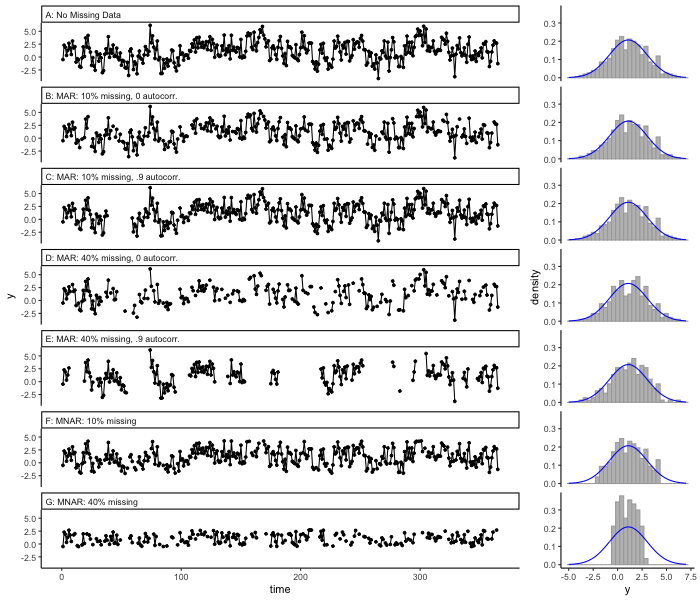
\includegraphics[width = 0.9\textwidth]{Figures/CompareMissingnessTypes_fig.png}
     \caption{An example time series demonstrating different types and amounts of missing data. Left column shows the same time series with different amounts and types of missingness and right column shows the distribution of data points in each resultant time series. A. Complete time series with no missing data. Rows B through E show the time series with 10\% (B and C) or 40\% (D and E) of data missing at random and with low autocorrelation in missing data (B and D) and high autocorrelation (C and E). Rows F and G show the time series with data missing not at random for 10\% missing data (F) and 40\% missing data (G).}
     \label{fig:missingtypes}
 \end{figure}



%% Figure 2
\begin{figure}[h]
     \noindent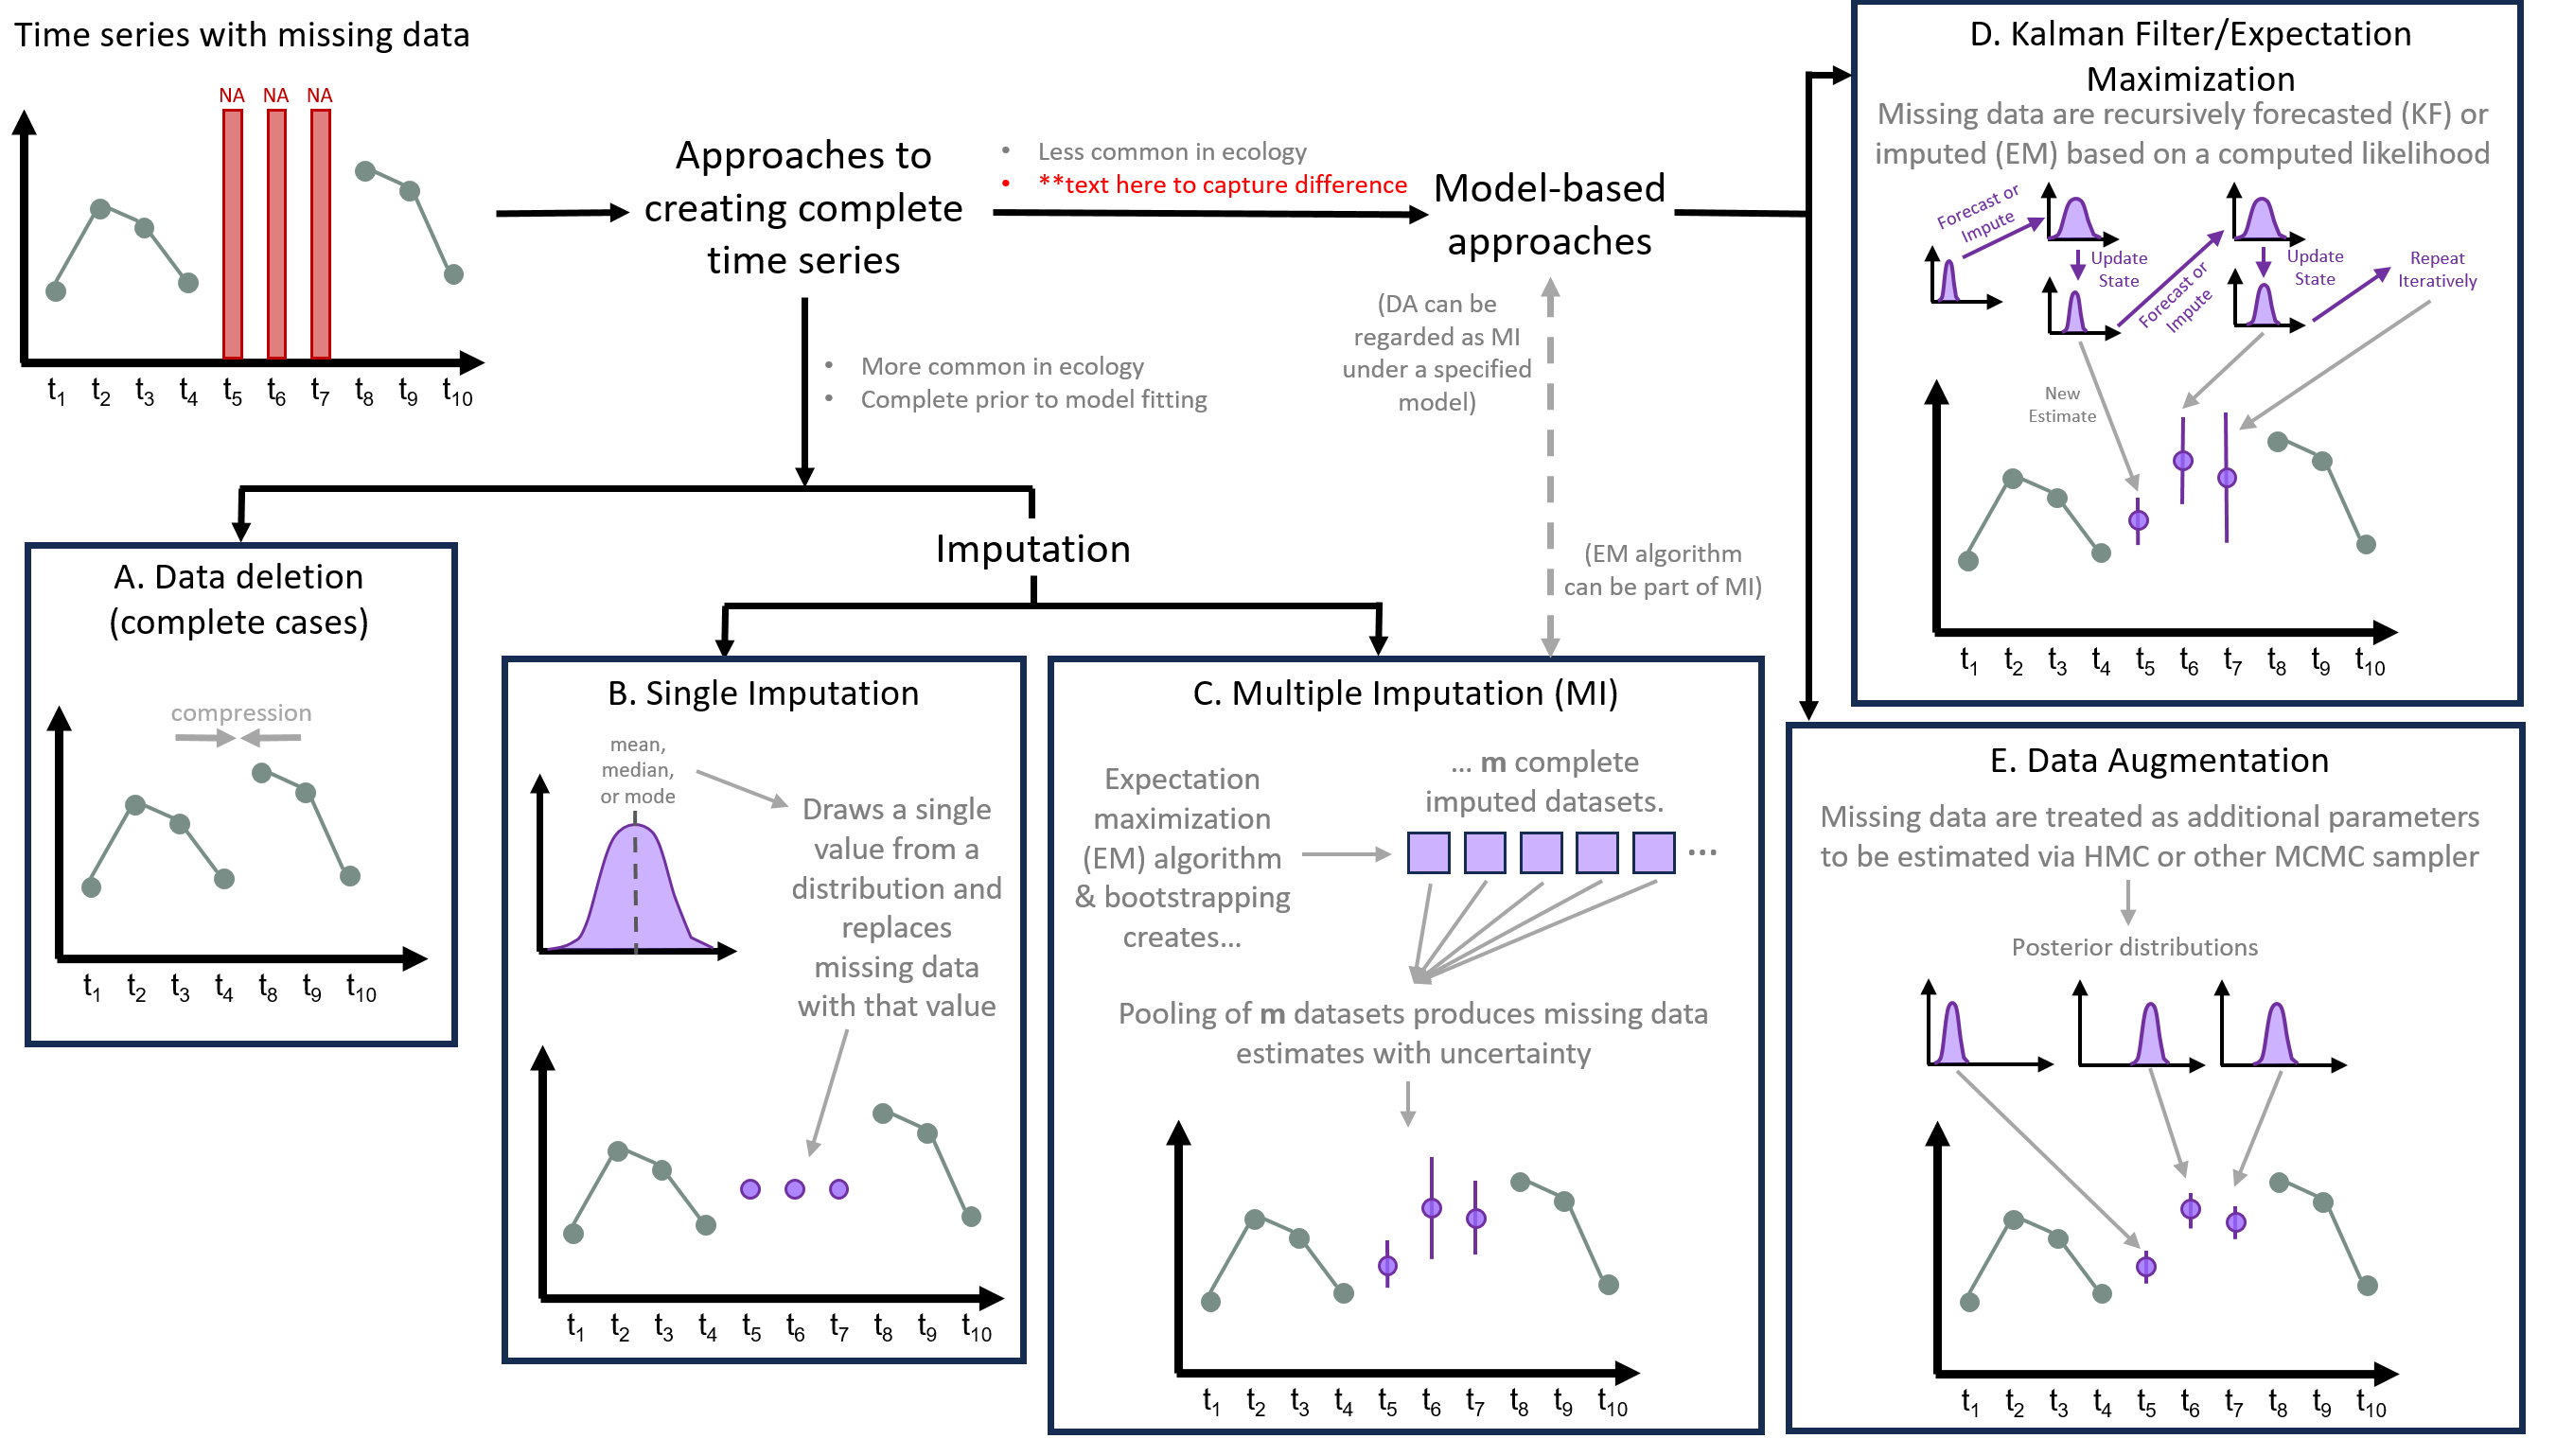
\includegraphics[width = 0.9\textwidth]{Figures/ConceptualFigure.png}
     \caption{Conceptual figure showing different approaches to handling missing data and the mechanisms for each approach}
     \label{fig:ConceptualFigure}
 \end{figure}

%% Figure 3
\begin{figure}
    \noindent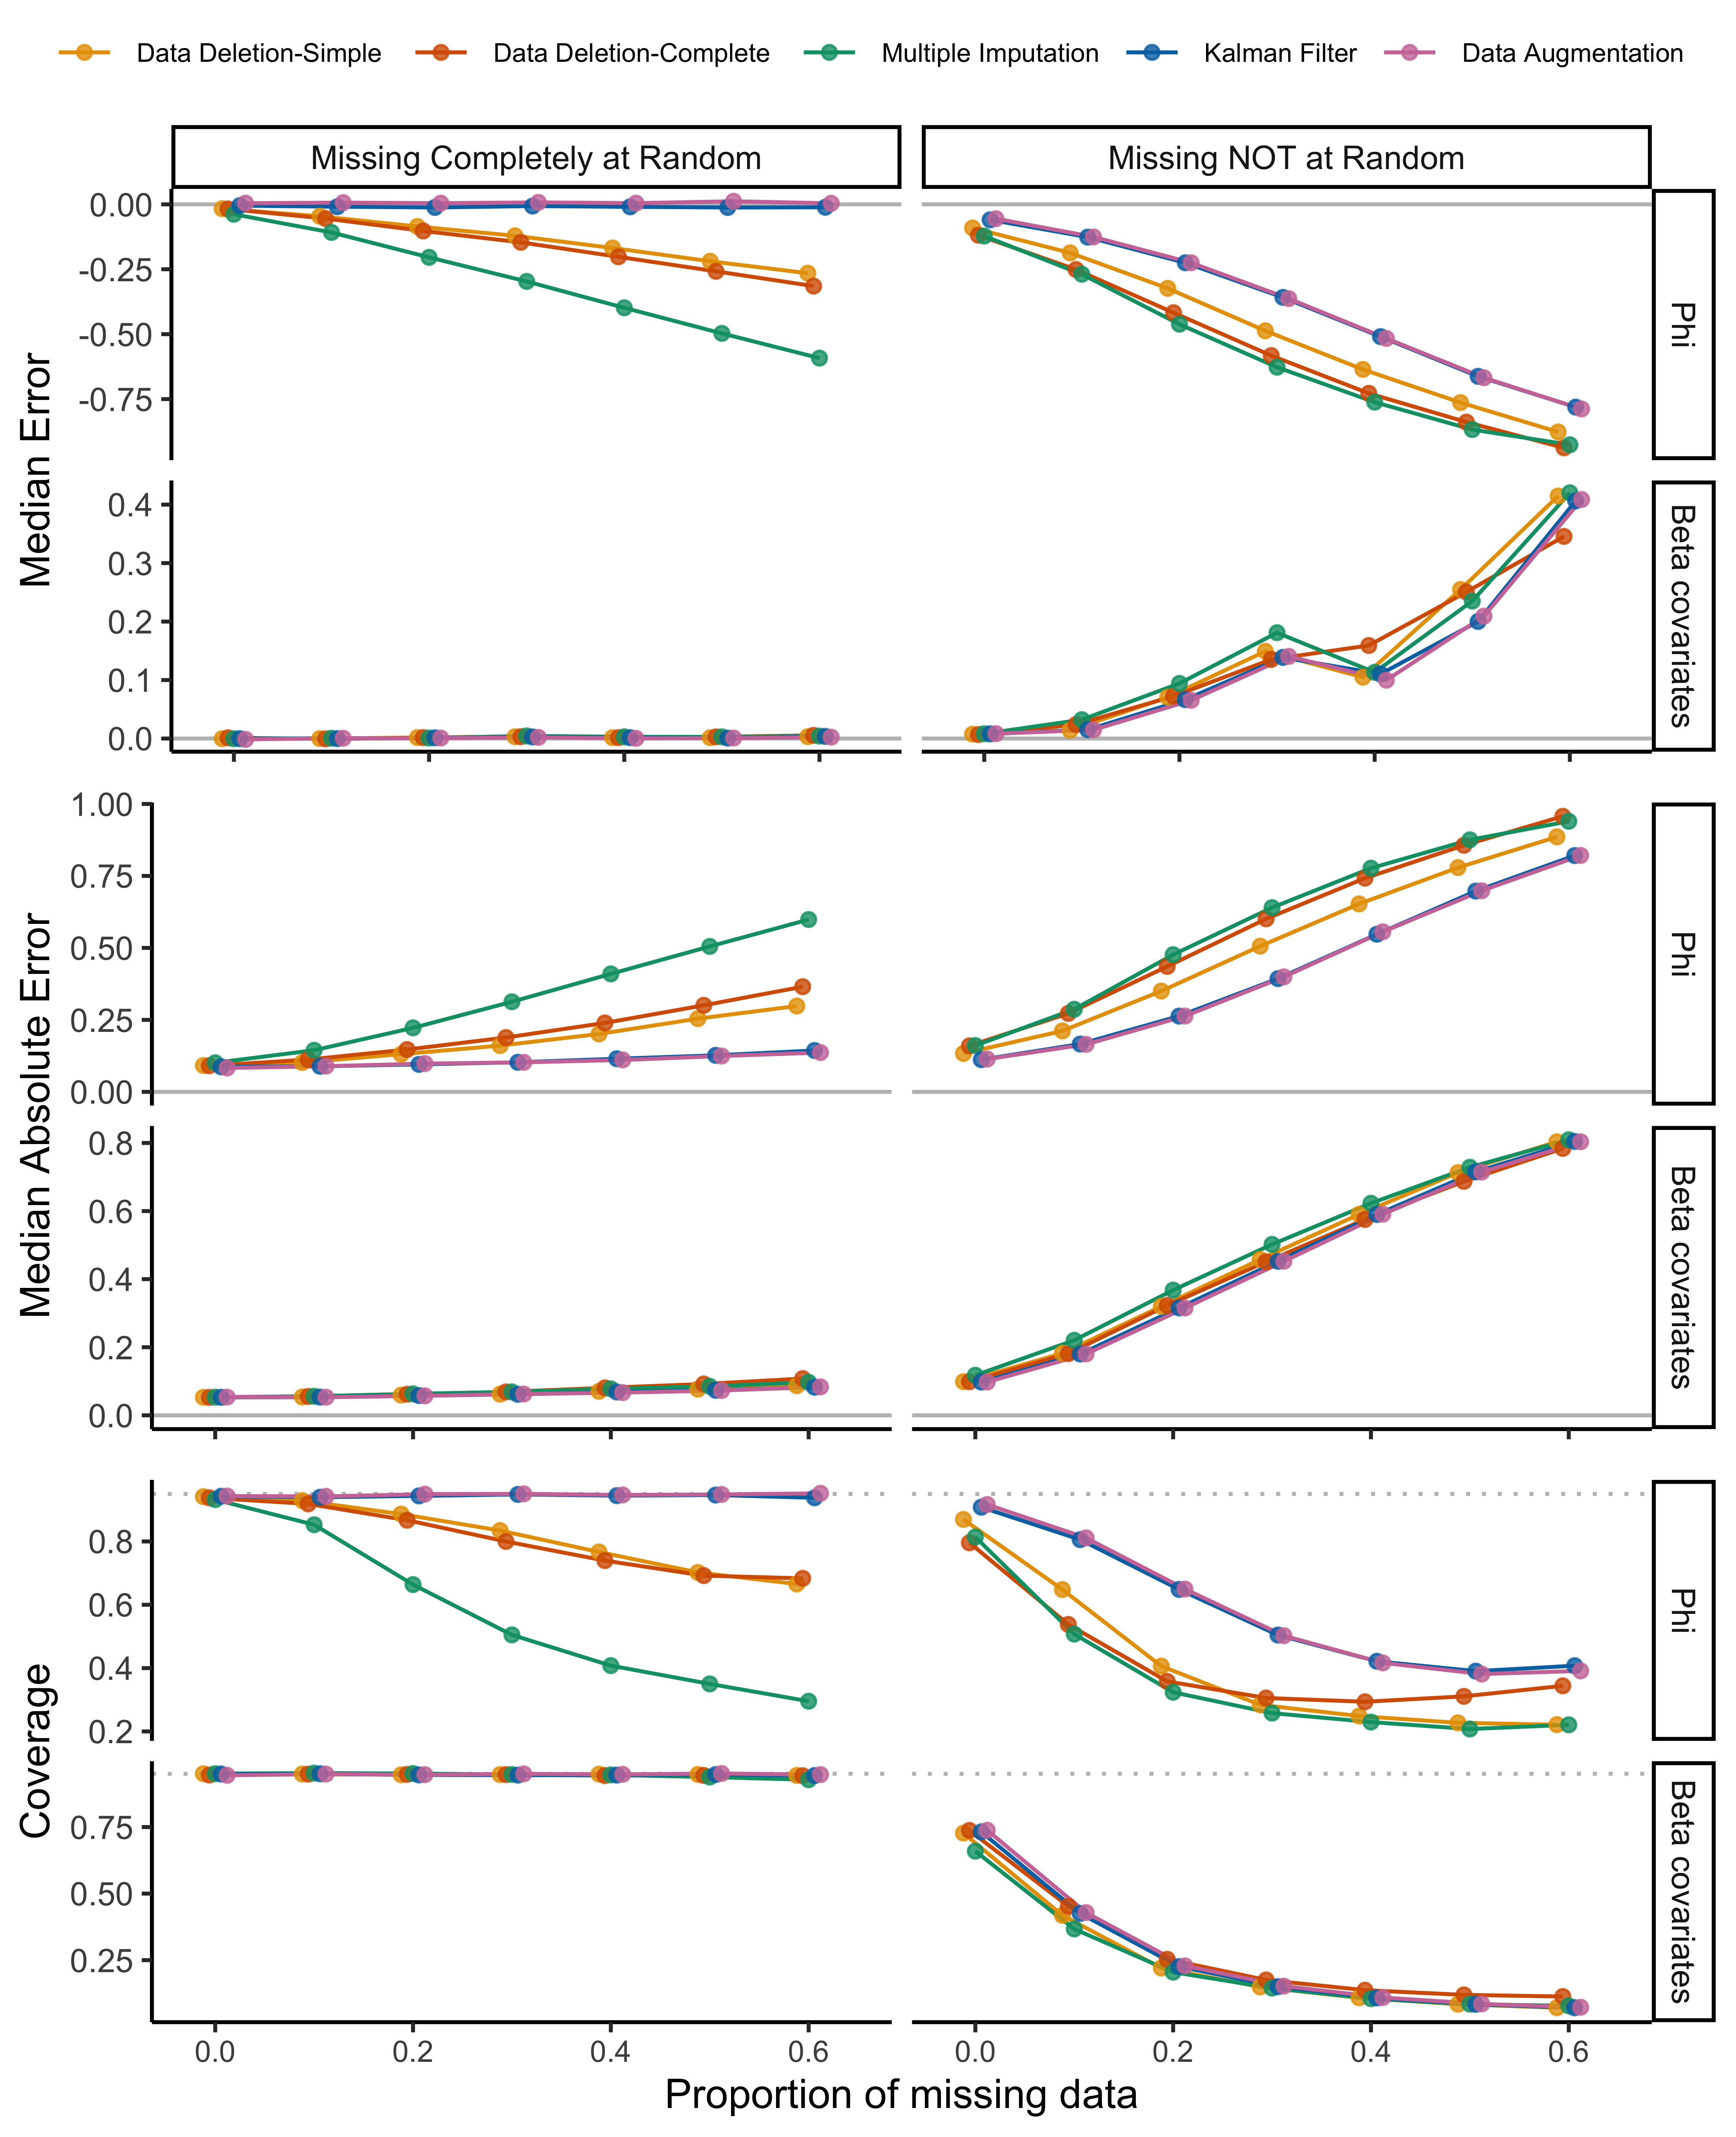
\includegraphics[width = \textwidth]{Figures/MockedUpFigures/parameterRecoveryGaussian_MARMNARlong.png}
    \caption{Parameter recovery metrics for Gaussian time series: Medians of parameter recovery, absolute error, and 95\% coverage of parameter estimates recovered using five methods of handling missing data across an increasing proportion of missing data. These analyses used simulated Gaussian datasets with data missing at random (MAR; left panel) and autocorrelation in missingness levels between $>$0.3 and $<$ 0.6, and data missing not at random (MNAR; right panel). The coverage panel shows the proportion of model runs where the 95\% confidence interval of a parameter estimate includes the true simulation parameter (dotted line at 0.95)}
    \label{fig:ParamRec_Gauss}
\end{figure}

%% Figure 4
\begin{figure}
    \noindent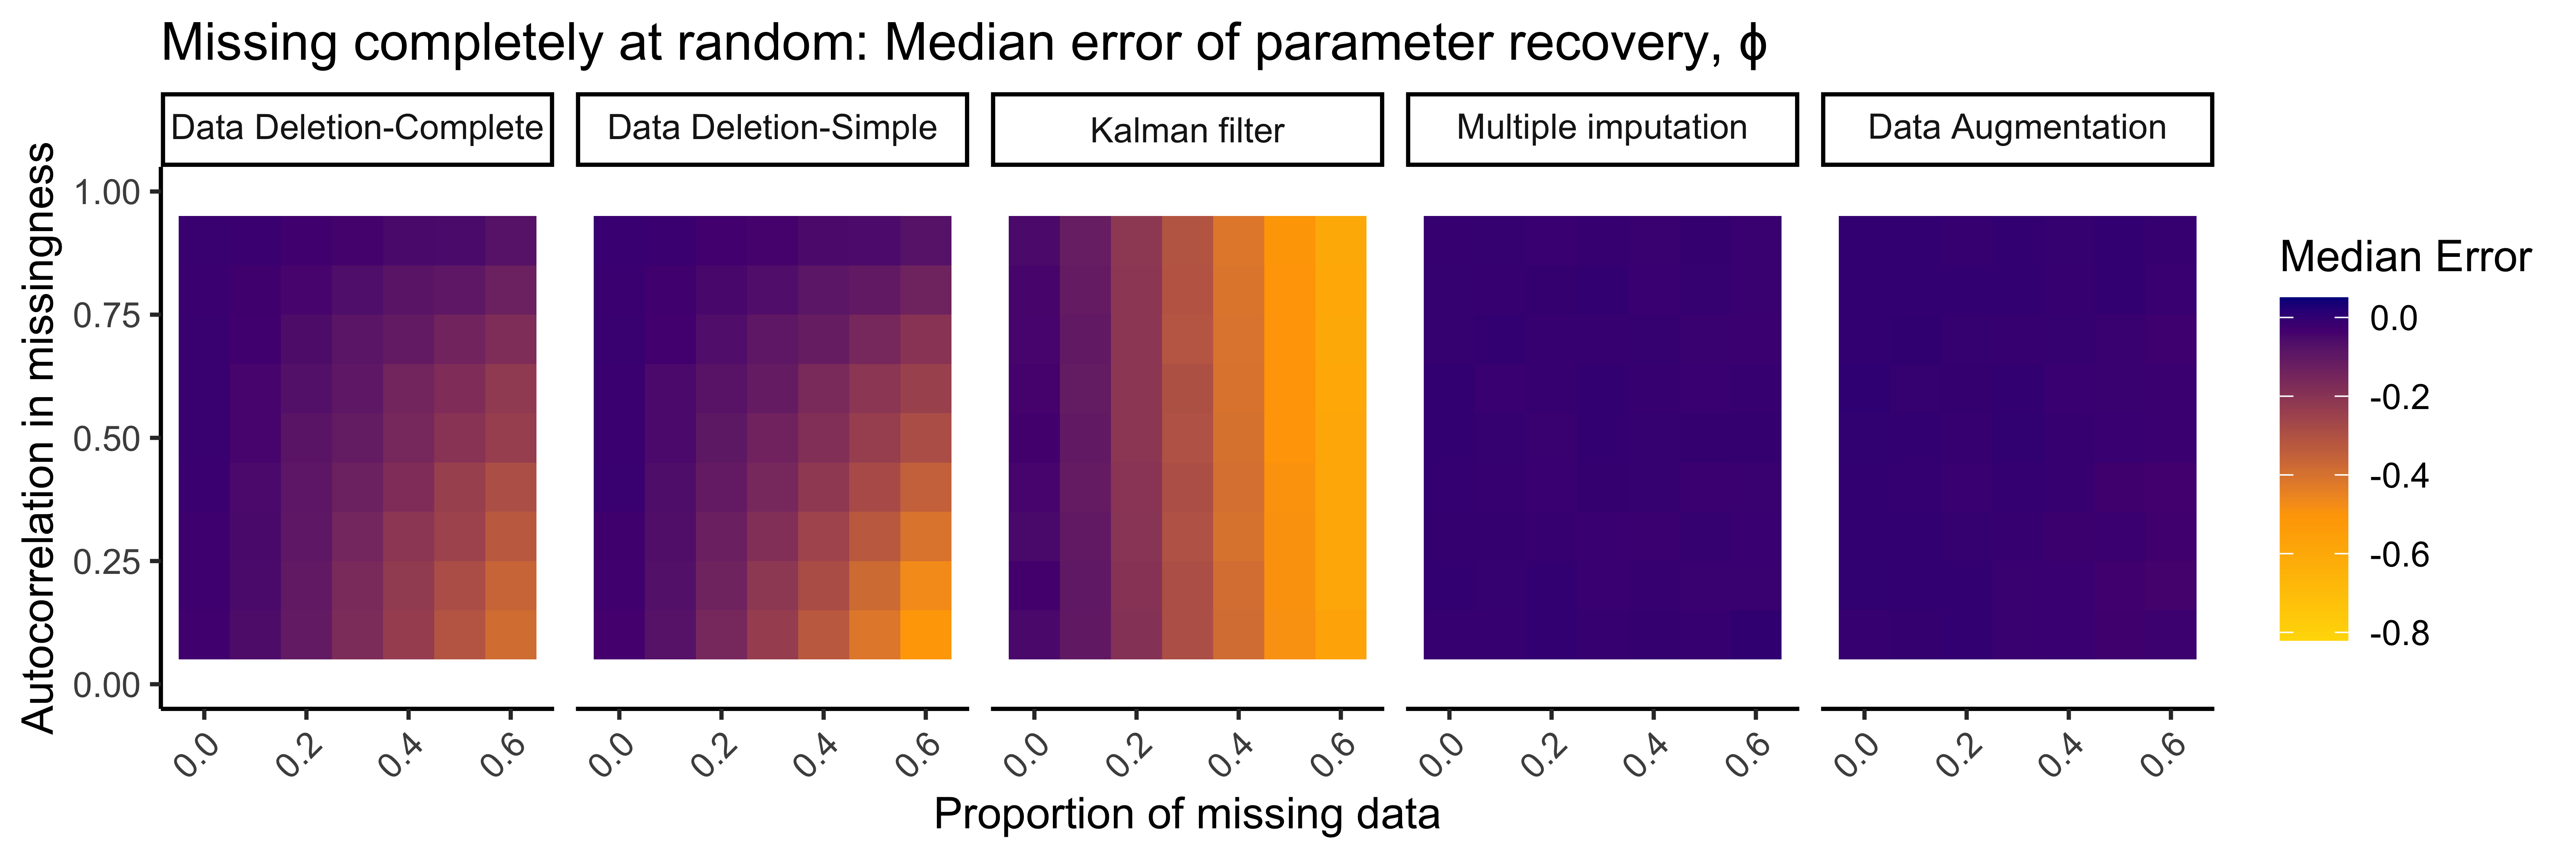
\includegraphics[width = \textwidth]{Figures/MockedUpFigures/heatmap_GaussianMCAR_justPhi.png}
    \caption{Median bias of $\phi$ standardized parameter recovery based on the proportion of missing data and autocorrelation in missingness recovered using five methods of handling missing data, using simulated Gaussian datasets with data missing at random (MAR). Cells in yellow (closer to 0) show model estimates closer to the actual parameter.}
    \label{fig:heatMap_gauss_MAR}
\end{figure}

%% Figure 5
\begin{figure}
    \centering
    \noindent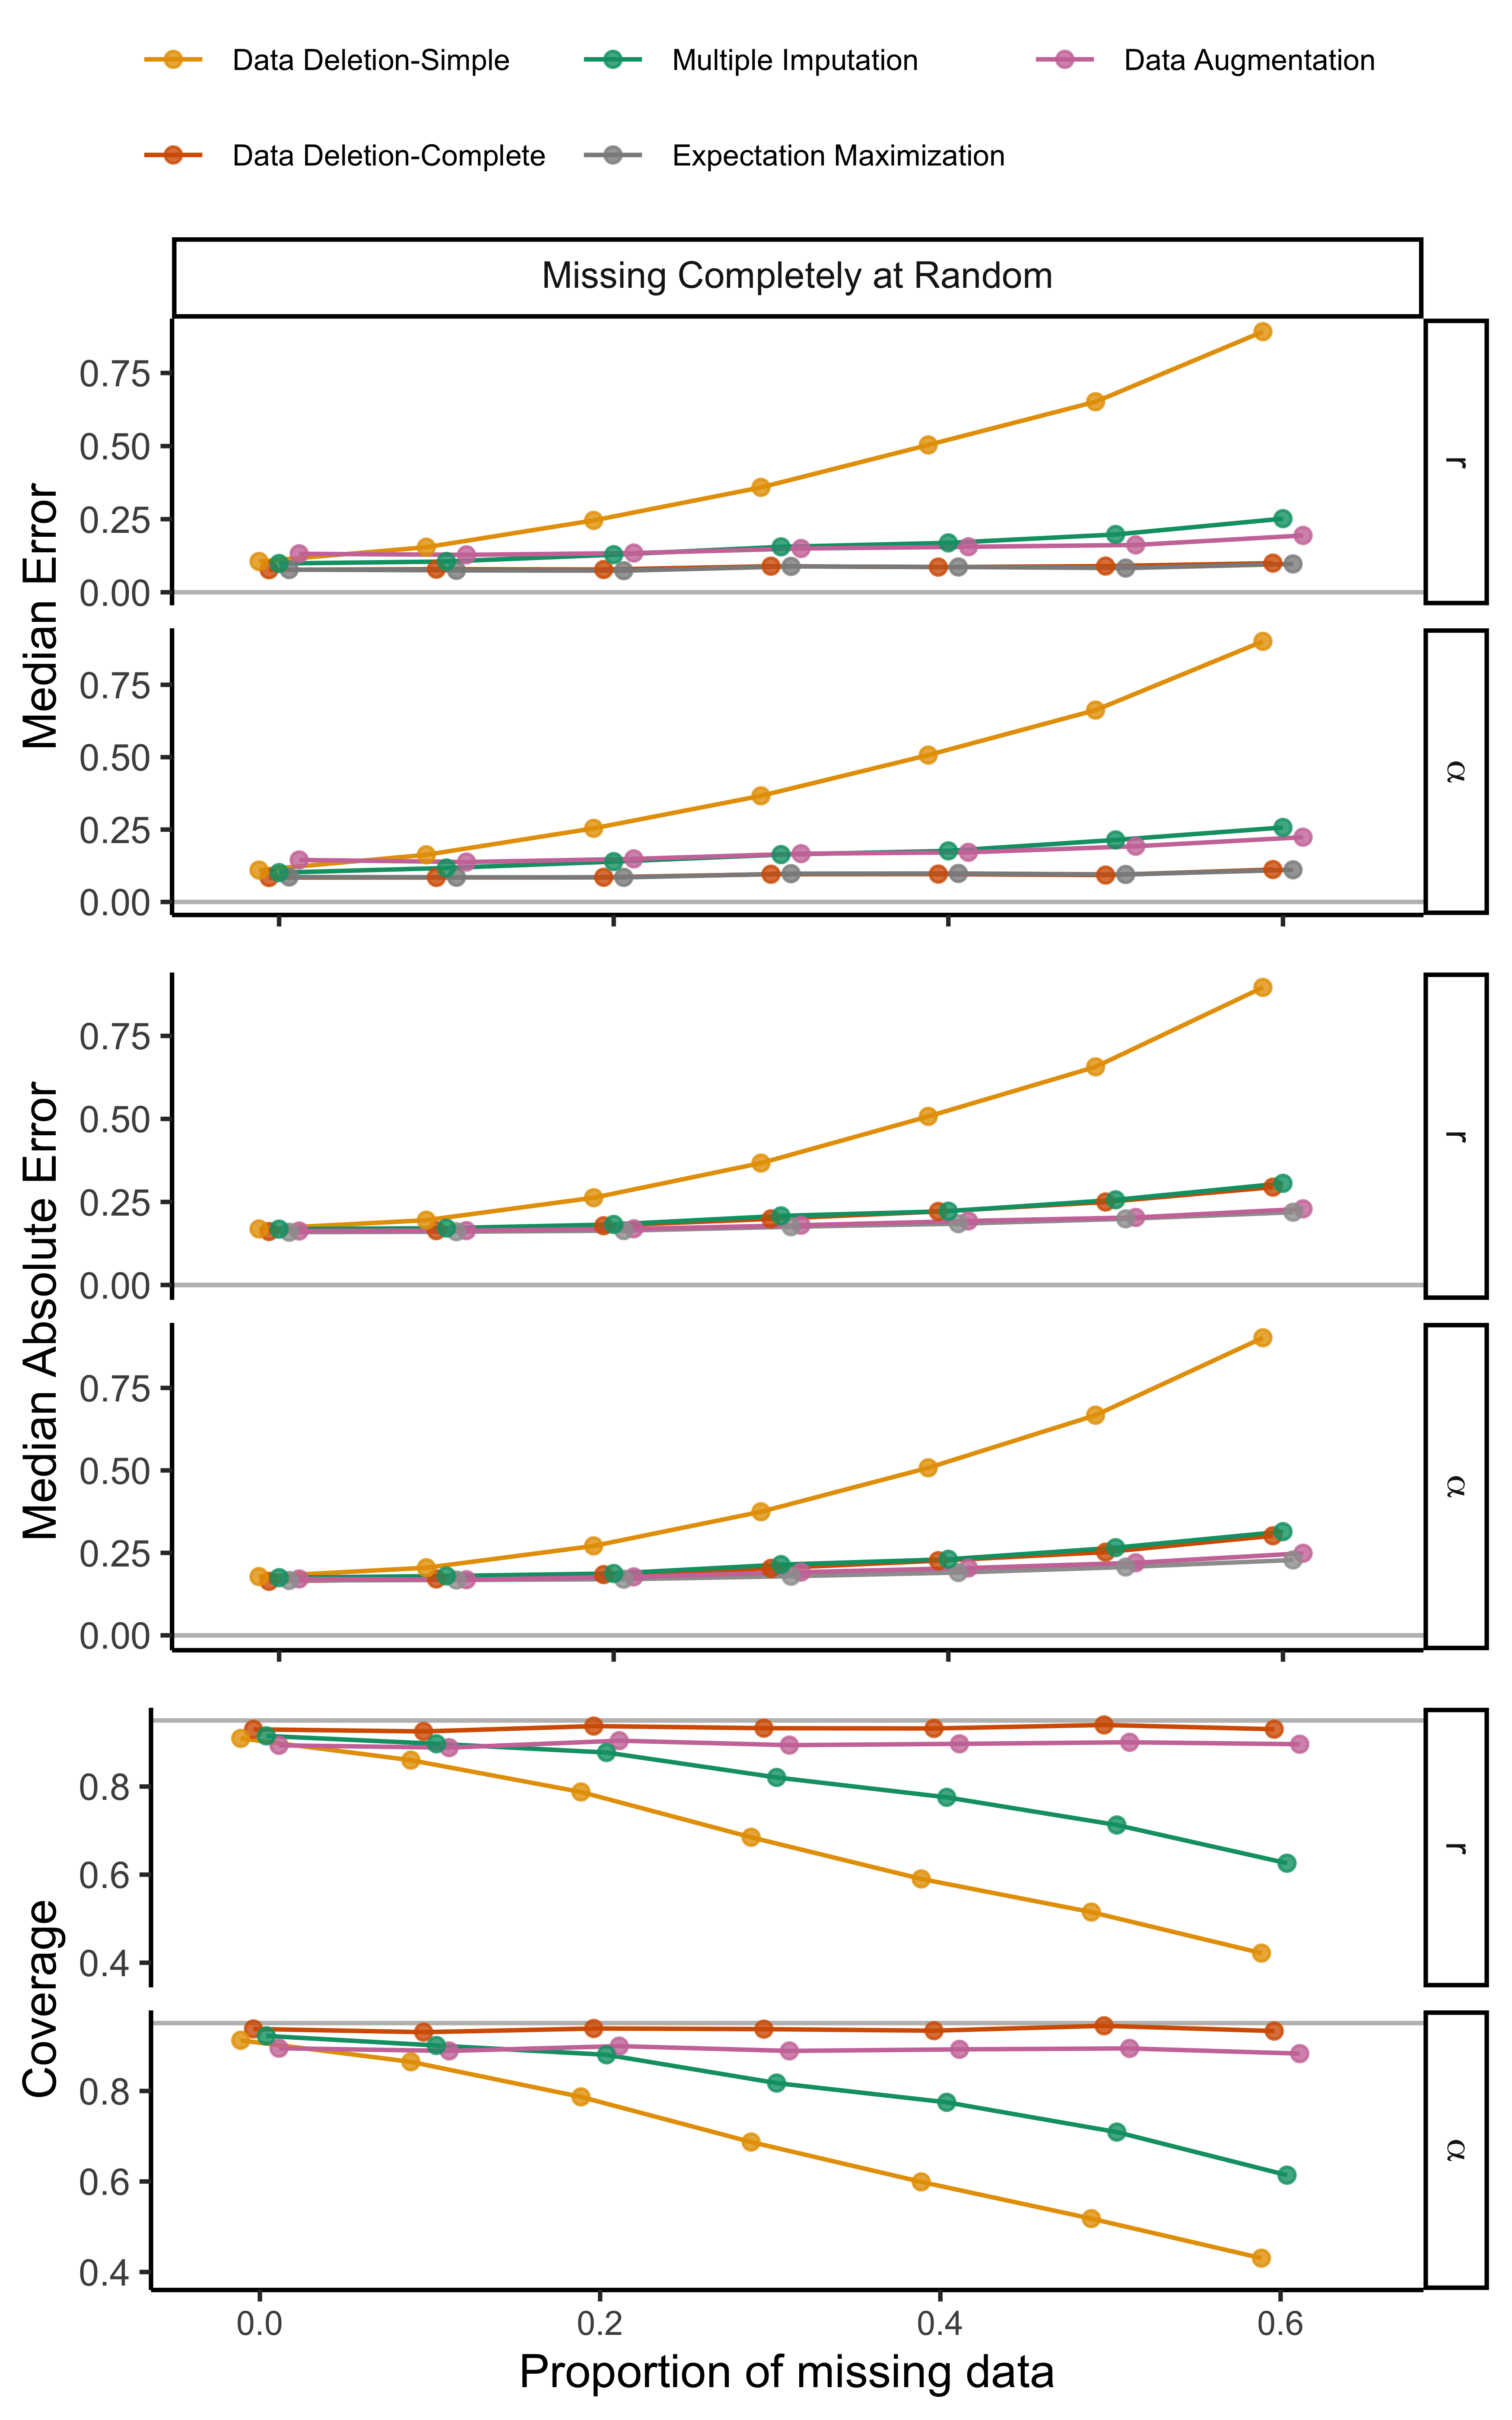
\includegraphics[width = 0.8\textwidth]{Figures/MockedUpFigures/parameterRecoveryPoisson_MCARlong.png}
    \caption{Parameter recovery metrics for Poisson time series: Medians of parameter estimate recovery, absolute error, and 95\% coverage of parameter estimates recovered using five methods of handling missing data across an increasing proportion of missing data, using simulated Poisson datasets where data were missing at random (MAR). The coverage panel shows the proportion of model runs where the 95\% confidence interval of a parameter estimate includes the true simulation parameter (dotted line at 0.95)}
    \label{fig:ParamRec_Pois}
\end{figure}

%% Figure 6
\begin{figure}
    \centering
    \noindent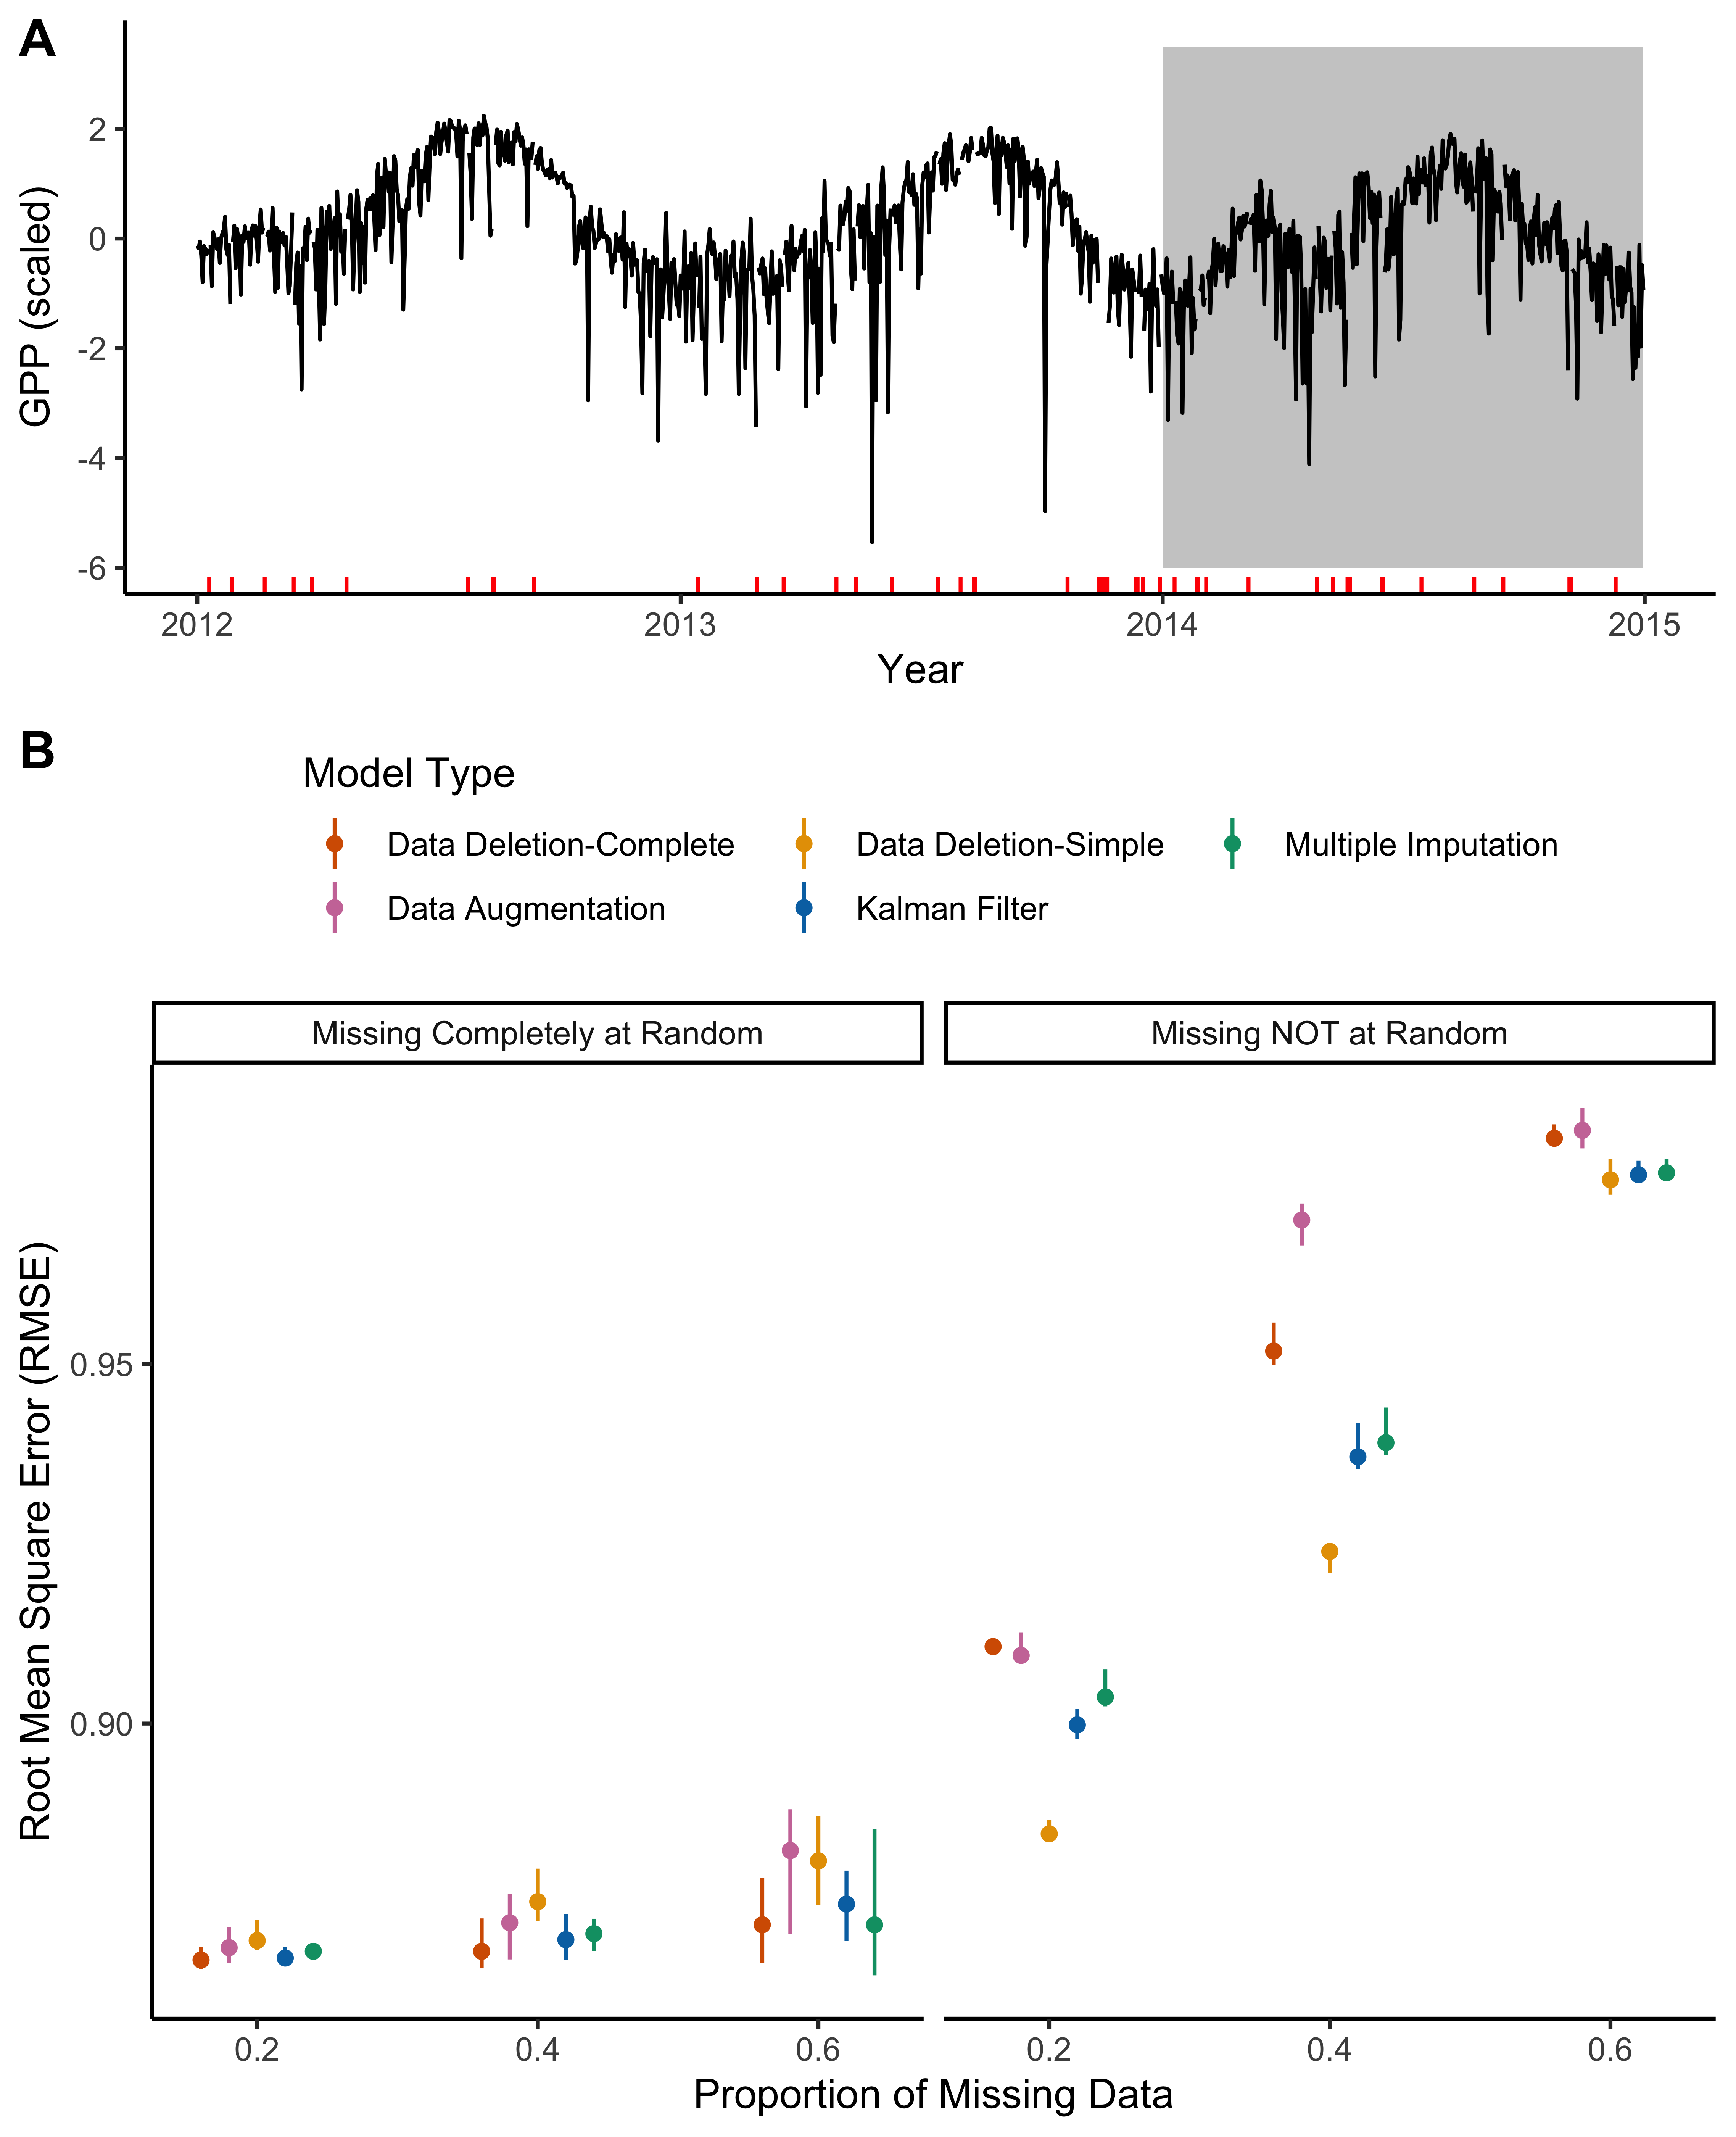
\includegraphics[width = 0.85\textwidth]{Figures/MockedUpFigures/RMSE_FullFigure_NoLineWithErrorBar_gaussian_auSable.png}
    \caption{(A) Daily measurements of scaled gross primary productivity (GPP) from the Au Sable River from 2012 through 2015 (699 days). Red tick marks on the x-axis indicate days when measurements were missing. The gray box indicates the data (347 days) excluded from model fitting, which were then forecast using the resulting model. (B) Root mean square error (RMSE) of forecasts made using a model fit to the Au Sable GPP time series shown in panel A. Each point shows the median RMSE across all forecasts with a given missing data approach (indicated by color), in a given level of proportion of missing data (0.2 $\pm$ 0.05, 0.4 $\pm$ 0.05, 0.6 $\pm$ 0.05), and with a given type of missingness (missing at random (MAR) with autocorrelation 0.5 $\pm$ 0.05 or missing not at random (MNAR)). Error bars indicate the inter-quartile range.}
    \label{fig:RMSE_Gaus}
\end{figure}

%% Figure 7
\begin{figure}
    \noindent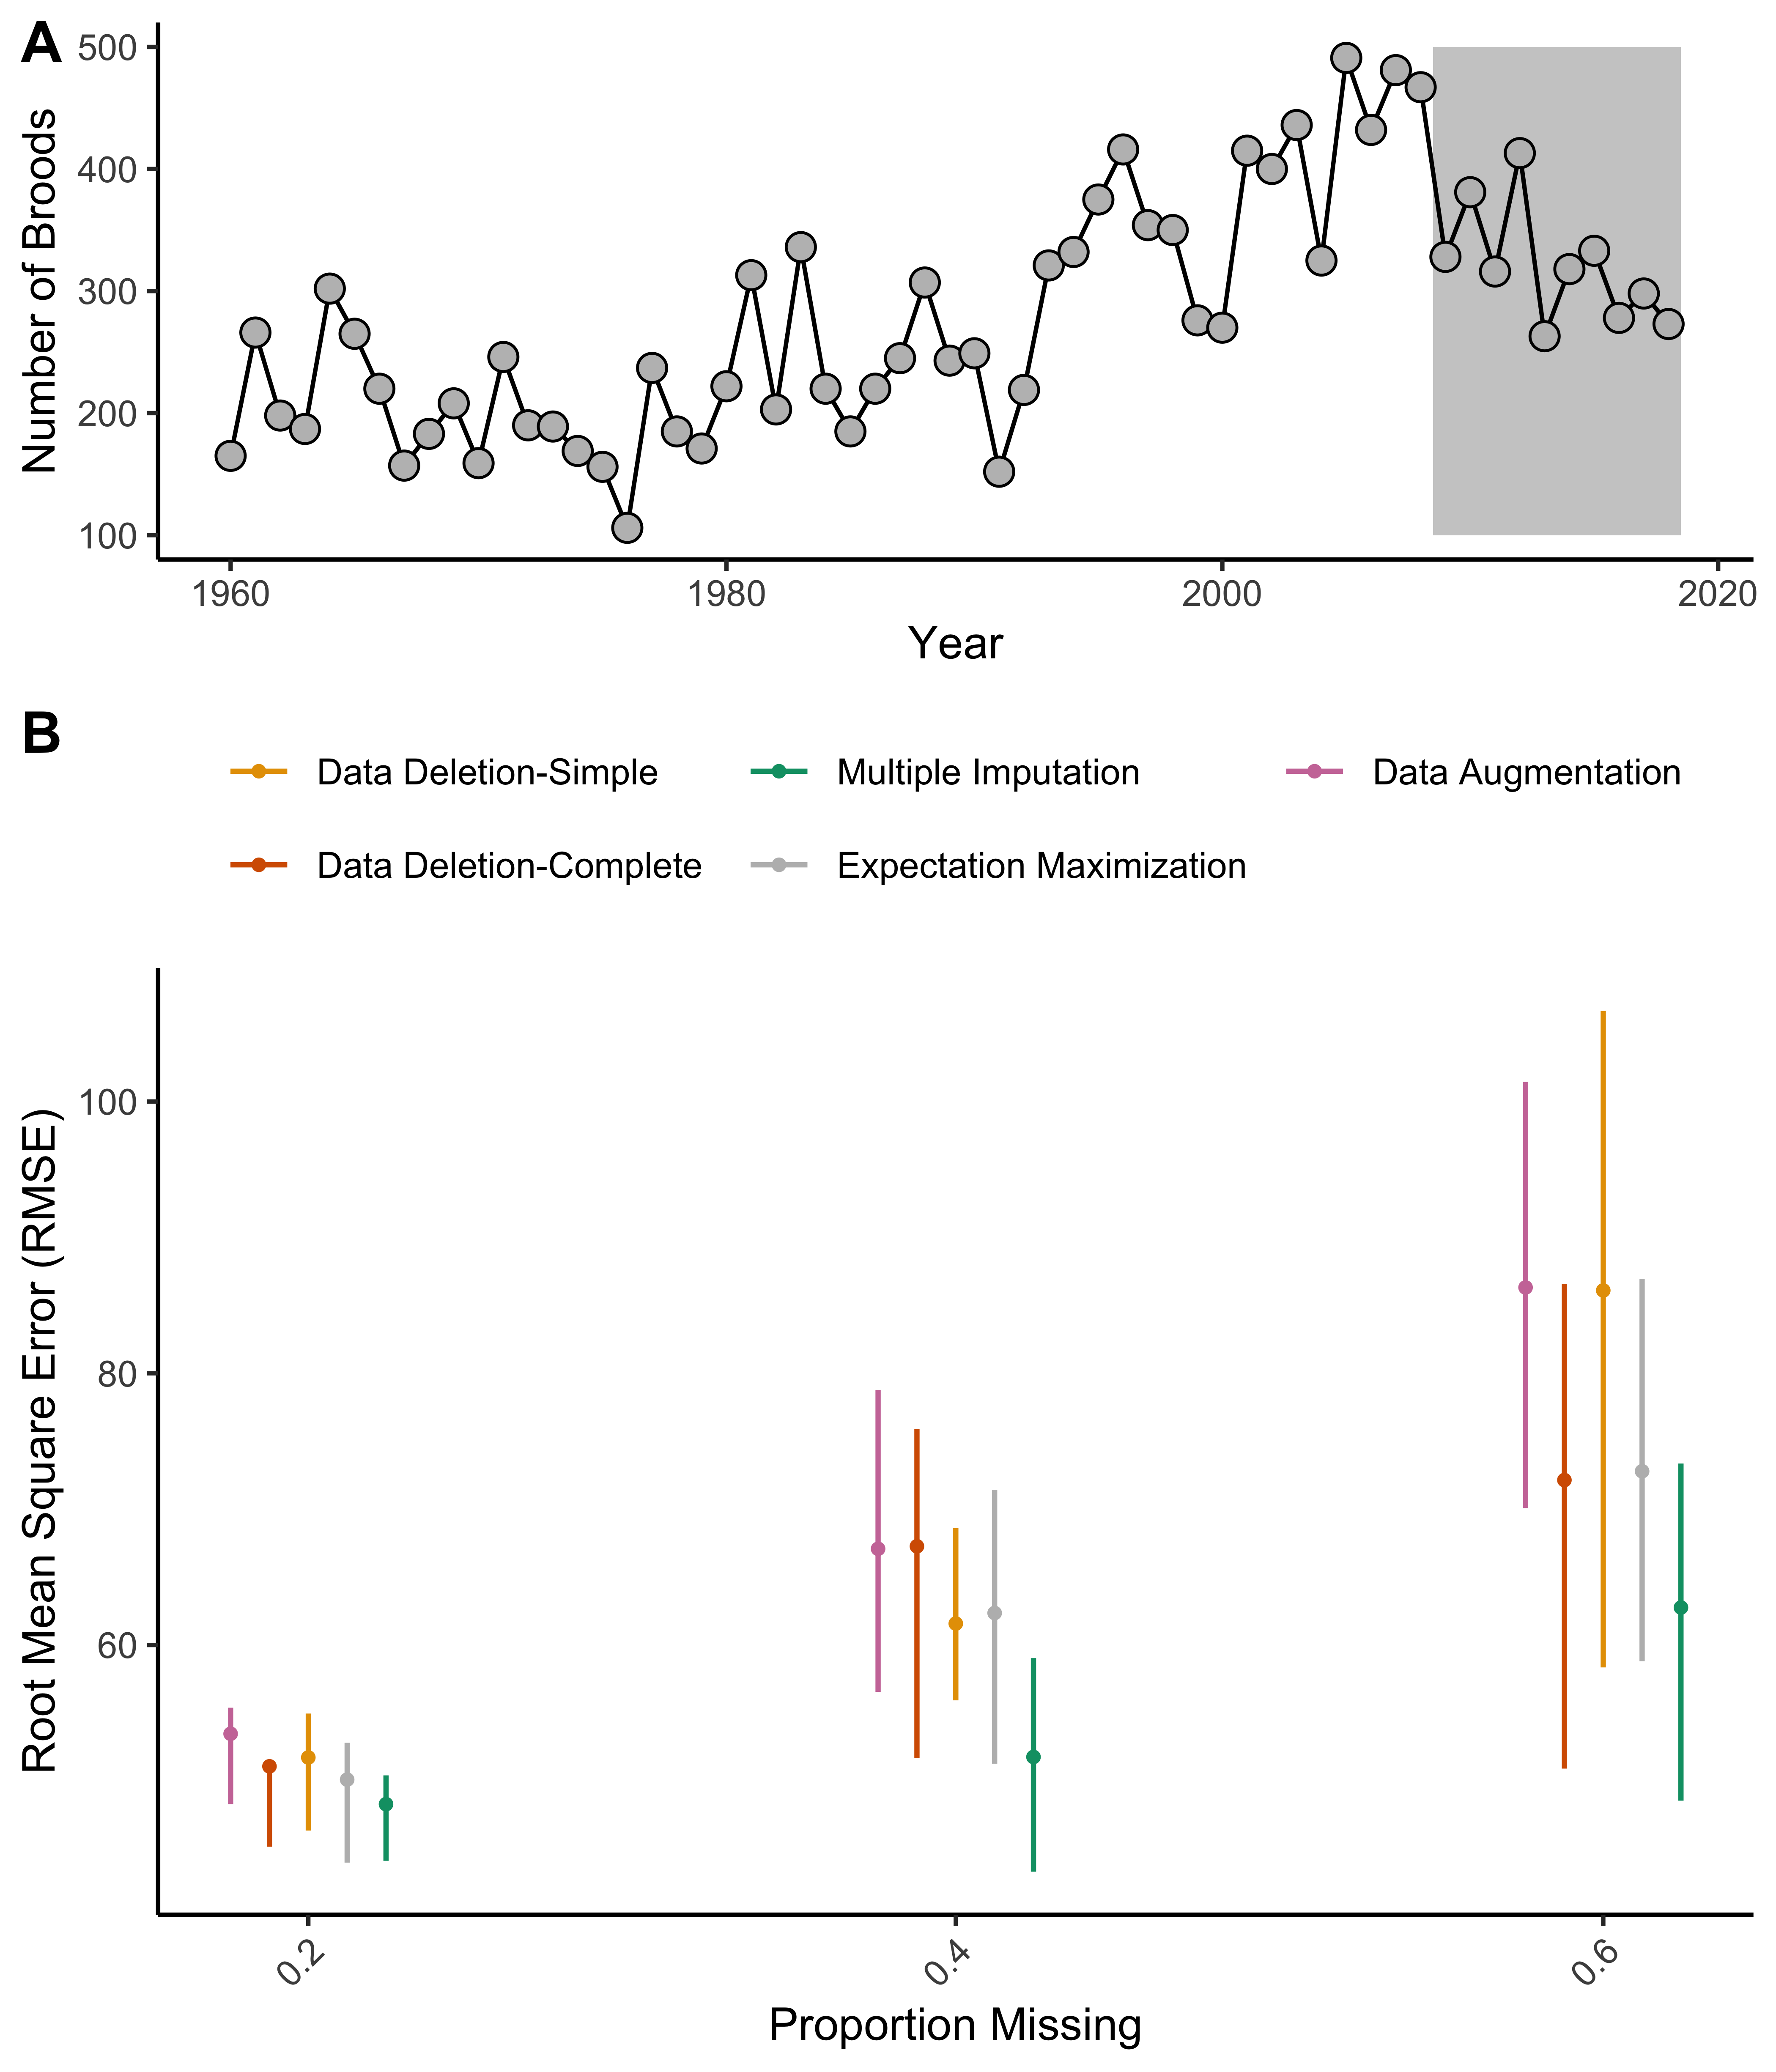
\includegraphics[width = \textwidth]{Figures/MockedUpFigures/RMSE_pois_combined.png}
    \caption{(A) Annual counts of Great Tit (\textit{Parus major}) broods in the Wytham Woods from 1960 – 2018. The gray box indicates the data (10 years) that were excluded from model fitting, which were then forecast using the resulting model. (B) Forecast root mean square error (RMSE) of the Great Tit dataset with an increasing proportion of missing data and missingness approaches. Each point shows the mean RMSE across all forecasts with a given missing data approach (indicated by color), in a given level of proportion of missing data (0.2 $\pm$ 0.05, 0.4 $\pm$ 0.05, 0.6 $\pm$ 0.05) with all bars shown for autocorrelation of 0.5 $\pm$ 0.05. Error bars indicate inter-quartile range}
    \label{fig:RMSE_Poiss}
\end{figure}
\clearpage


\newpage

\bibliographystyle{ecology}
\bibliography{citations}

\newpage

%%\appendix
\documentclass[12pt,english]{article} %12 pt for Ecology %
\usepackage[utf8]{inputenc}

\usepackage{geometry}                		
\geometry{verbose,letterpaper,tmargin=2.54cm,bmargin=2.54cm,lmargin=2.54cm,rmargin=2.54cm}   % 1 inch margins for Ecology   

\usepackage{multirow}
\usepackage{graphicx}		
\graphicspath{ {c:} }
\usepackage{setspace}
\usepackage[version=4]{mhchem}
\doublespace
\usepackage{siunitx}
\usepackage[
  backend=biber,
  style=apa,
  maxcitenames=2,
  natbib=true]{biblatex}
\addbibresource{citations.bib}
\usepackage{amsmath}
\usepackage{bm}
\usepackage{amsfonts}
\usepackage{lineno}
\usepackage{gensymb}
\usepackage[sharp]{easylist}%makes nice outlines.  Use # for symbol
\usepackage{blkarray}
\usepackage{lastpage}
\usepackage{times} % times new roman%
\usepackage{lineno} % add line numbers%

\begin{document}


\noindent\textbf{Journal}: Ecology; \textbf{Article Type}: Statistical Innovations

{\Large \noindent \bf %Approaches for handling missing data in ecological time series
Accounting for missing data in autoregressive models of ecological time series
}

%Journal name
%Manuscript type

\medskip

\noindent Alice E. Stears\textsuperscript{*, 1, 2}, 
Melissa DeSiervo\textsuperscript{*, 3, 2},
Dustin Gannon\textsuperscript{4, 2},
Amy Patterson\textsuperscript{5, 2},
Alice M. Carter\textsuperscript{6,7},
Joanna R. Blaszczak\textsuperscript{8},
Matt Trentman\textsuperscript{9},
Eliza Grames\textsuperscript{10},
Robert O. Hall, Jr\textsuperscript{7},
Joshua P. Jahner\textsuperscript{11, 2},
Saheed O. Jimoh\textsuperscript{2},
Courtenay A. Ray\textsuperscript{2},
Christa L. Torrens\textsuperscript{7},
Lauren Shoemaker$^{\circ}$\textsuperscript{2},
Christopher Weiss-Lehman$^{\circ}$\textsuperscript{2}

\noindent\noindent \textbf{Author affiliations}

\noindent\textsuperscript{1} Center for Adaptable Western Landscapes, Northern Arizona University, Flagstaff, AZ

\noindent\textsuperscript{2} Botany Department, University of Wyoming, Laramie, WY

\noindent\textsuperscript{3} Biology Department, Union College, Schenectady, NY

\noindent\textsuperscript{4} Department of Forest Ecosystems and Society, Oregon State University, Corvallis, OR 

\noindent\textsuperscript{5} Department of Biology, University of Maryland, College Park, MD

\noindent\textsuperscript{6} Department of Mathematics and Statistics, Utah State University, Logan, UT

\noindent\textsuperscript{7} Flathead Lake Biological Station, University of Montana, Polson, MT

\noindent\textsuperscript{8} Department of Natural Resources and Environmental Sciences, University of Nevada, Reno, Reno, NV

\noindent\textsuperscript{9} O’Connor Center for the Rocky Mountain West, University of Montana, Missoula, MT

\noindent\textsuperscript{10} Biological Sciences, Binghamton University, State University of New York, Binghamton, NY

\noindent\textsuperscript{11} Department of Biology, New Mexico Institute of Mining and Technology, Socorro, NM

\noindent\textsuperscript{*} Denotes equal contribution as lead author

\noindent{$^{\circ}$} Denotes equal contribution as primary investigator

\noindent \textbf{Corresponding author}: Alice Stears, alice.e.stears@gmail.com 


\section*{Appendix S1}


\subsection*{Introducing Missingness}

We created MCAR datasets with varying proportions of missing data and degrees of autocorrelation in missingness (Fig. \ref{fig:missingtypes} B--E) by viewing a time series as a Markov-modulated Bernoulli process where the variable could have two states: missing or not missing \citep{Gharib2014, Edwards1960}. The probability that an observation in a time series at time $t+1$ was missing depended on both the specified proportion of non-missing values in the entire time series ($p$) and the specified degree of autocorrelation in missingness ($\omega$). In a time series $X_1, X_2, ..., X_n$, the transition matrix that describes the probability of an observation at $X_{t+1}$ being missing, based on whether the observation at $X_t$ was missing is defined as: 


\begin{equation}
\begin{blockarray}{rcccc}
\text{} & \BAmulticolumn{4}{c}{X_{t+1}}\\
X_t & \text{Present} & \text{Missing}  \\
\begin{block}{r(cccc)}
\text{Present} & 1-(1-\omega)p & (1-\omega)p \\
\text{Missing} & (1-\omega)(1-p) & \omega + (1-\omega)p  \\
[1ex]
\end{block}
\end{blockarray}
\end{equation}


We created MNAR datasets with various proportions of msising data by first calculating the mean and standard deviation of the time series with no missing data, then using these point estimates as the mean and standard deviation of a normal distribution. We then identified the quantiles of that normal distribution above and below which the density of the normal distribution corresponded to the desired proportion of missingness. We replaced any values above and below those quantiles with an NA.

\subsection*{Missing Data Approaches} 
\textbf{Simple and Complete Data Deletion}: The ``simple data deletion" approach involves removing missing values from a time series, compressing the dataset, and running the model as if the time intervals between observations were all equal (Fig. 1 A). This method violates the assumption of equal temporal spacing between observations, an assumption implicit in most time series models. We include it here as a reference because it is simple and commonly used in published studies. We also include ``complete case data deletion," which maintains equal spacing between observations by removing a missing value itself as well as the subsequent observation(s) that is predicted by the missing value (Fig. 1 A). However, those observations after a missing value are retained as predictors of the subsequent observation(s). 

\textbf{Multiple Imputation}: Multiple imputation (MI) is an approach that systematically fills in missing observations with imputed values, and creates several versions of complete data sets that can be used to estimate uncertainty around each imputed value (Fig. 1 B). MI is commonly used in ecology, with multiple studies evaluating methods and approaches to conduct MI for functional traits \citep{taugourdeau_filling_2014,johnson_handling_2021,penone_imputation_2014}, population biology \citep{onkelinx_working_2017}, time series \citep{hui_gap-filling_2004}, and meta-analyses \citep{ellington_using_2015}. Multiple Imputation’s (MI) effectiveness can depend on the number of imputed datasets (\textit{m}). It is often assumed that \textit{m}=5 is a minimum value \citep{honaker_what_2010}; however, researchers have used \textit{m}=200 when comparing methods in the ecological sciences \citep{onkelinx_working_2017}. In general, larger values of \textit{m} result in more accurate estimates of both parameter values and uncertainty. However, increasing \textit{m} results in a trade-off between accuracy and computation time; this can be particularly problematic for data-rich (e.g., long time series) or complex (e.g., hierarchical) models. 
After imputing the \textit{m} data sets, the analyses of interest are confronted with each data set, and the estimated parameters from the \textit{m} analyses are averaged using Rubin rules of averaging to get the parameter(s), and associated uncertainty, from which inference can be made. We implemented multiple imputation with the Amelia II package in R \citep{honaker2011}, which uses an expectation maximization algorithm (see below) in combination with a bootstrapping technique for deciding what values to impute. We used $m=5$ in order to provide decent estimates without excessive run times.

For both the simulated and empirical population count time series, since we did not have any covariates, the only variables used for imputation were the population size at time \textit{t} and population size at time \textit{t-1}. For time series with chunks of missing data, the Amelia multiple imputation function had to be run iteratively, with missing values filled in from the edges of the missing chunks. In addition, while the recommended settings for dealing with time series data using the Amelia package include incorporating preceding and proceeding time points by specifying the ``lags" and ``leads" options \citep{honaker2011}, it was not possible to use the lags option, since the current population was already using the population at the previous point as its only predictor for imputation. Instead, we included only the leads option, which still resulted in occasional failure of the method at extremely high levels ($>70\%$) of missing data due to excessive collinearity between the preceding and proceeding time points. The lack of error handling for extremely collinear variables is an unfortunate issue for this method when using data sets without covariates, or data sets with highly collinear covariates.  

For both the simulated and empirical Gaussian series, implementing multiple imputation was more straightforward since an observation at time \textit{t} was informed by two covariates in addition to the observation at the time \textit{t-1}. In this case, we were able to use both the ``lags" and ``leads" options in \texttt{amelia}. 

Following execution of MI using Amelia II, we fit statistical models to time series following the methods described in \textbf{Main Text: Comparing missing data approaches}.

\textbf{Kalman Filter}: The Kalman Filter (KF) was developed to estimate the state of a dynamic system that is observed with error but can be used to derive the likelihood function of a time series with missing observations (Fig. 1 C). To illustrate the approach, assume a state-space model

\begin{equation}
    \begin{aligned}
        X_t &= \phi X_{t-1} + \epsilon_t \\Y_t &= X_t + e_t
    \end{aligned}
\end{equation}
where $X_t$ is the true ``state" of the system at time $t$, $Y_t$ is the observed value at time $t$, and $\epsilon_t \sim \mathcal{N}(0, \sigma^2)$ and $e_t \sim \mathcal{N}(0, \tau^2)$ are IID white noise error terms for the process and observation error, respectively. The Kalman Filter is primarily focused on estimating the unobserved state of the system, $X_t$, and can be conceptualized as a two-step procedure in which, given an initial state $X_0$, we can forecast the next state $X_1$. Then, following data collection at the next time point, $y_1$, we update the forecast using Bayes' theorem. Specifically, the forecast distribution for $X_1$ is
\begin{equation}
    p(x_1) = \int p(x_1 | x_0)p(x_0)dx_0
\end{equation}
where $p(\cdot)$ denotes the probability density function. Assuming IID Gaussian errors, $p(x_1)$ is normal with mean ${\tilde x}_1 = \phi x_0$ and variance $v_1 = \phi^2 \frac{\sigma^2}{1 - \phi^2} + \sigma^2$. Given the observed value $y_1$, we update the estimate of $X_1$ using Bayes theorem
\begin{equation}
    \begin{aligned}
        p(x_1 | y_1) &\propto p(y_1 | x_1) p(x_1)
        &= \mathcal{N}\Bigl(\tilde x_1 + K_1(y_1 - \tilde x_1),\ (1 - K_1)v_1 \Bigr)
    \end{aligned} 
\end{equation}
where $K_1 = v_1 / (v_1 + \tau^2)$ is the \textit{Kalman gain} and creates a weighted average of the forecast and observation. %If the observation error is large, the forecast is favored as an estimate of $X_t$, whereas if the process noise is large relative to the observation error, the estimate of $X_t$ tends towards the observed value $y_t$.
For our focus on missing data, we assume the process is observed without error such that $Y_t = X_t$ and $\tau^2 = 0$. Without observation error, the Kalman gain $K_t = 1$ for all $t$ since $\tau^2 = 0$, and $p(x_1 | y_1) = \mathcal{N}(y_t, 0)$. Thus, the update step gives complete information about $X_t$, and the likelihood function can be defined based on the data $y_1,...,y_n$. However, if data are missing, the update step cannot occur. So, in the case of missing data without observation error, the Kalman Filter alternates between pure forecast steps when data are missing and pure ``update" steps when data and the state of the system are completely observed, but the forecast steps yield a method for computing the likelihood function recursively without needing to know the states of $X_t$ in which we were unable to observe the process and therefore have no associated $y_t$.

The Kalman filter assumes a Gaussian error distribution, so we only used this method with the simulated and empirical real-valued time series. We implemented KF missing data approach at the same time as the model fitting process, where we fit an AR(1) model with two covariates using the \texttt{arima} function from the \texttt{stats} package in R \citep{r_2021} (KF is the default algorithm used to handle missing values in this R function). 


\textbf{Expectation Maximization}: The expectation maximization (EM) algorithm is an iterative algorithm that is conceptually similar to KF, and recursively computes the likelihood of a time series with missing data (Fig. 1 D). Given an initial guess for the parameter vector we wish to estimate, ${\bm \theta}_0$, the first step (Expectation step) proceeds to ``fill in" the missing observations with their expectation given the observed data and the initial parameter vector ${\bm \theta}_0$ %. For example, if $Y_t$ were missing, we impute $Y_t$ with $\mathbb{E}(Y_t | y_{t-1}, {\bm \theta}_0)$
, which is equivalent to the forecast step of the Kalman filter conditioned on ${\bm \theta}_0$. In the second step (maximization step), we compute the maximum likelihood estimate of ${\bm \theta}$ using the filled-in time series as data to give an updated estimate $\hat {\bm \theta}_1$. We then iterate this process, updating the forecasts of the missing data using their expectations conditional on $\hat {\bm \theta}_1$, then maximizing the likelihood with respect to $\bm \theta$ using the time series filled-in with the updated forecasts. This process is iterated until the difference between successive estimates is acceptably small, indicating convergence (that is, $||\hat {\bm \theta}_i - \hat {\bm \theta}_{i-1}||_1 < \delta$ for some small $\delta > 0$).

Given its similarity to KF, we only used this missing data approach for the simulated and empirical times series of counts. We constructed an approximate EM algorithm to estimate the parameters of the Ricker model in which missing data were rounded to the nearest integer value during the expectation step such that the likelihood was well-defined for the filled-in series. As such, the missing data were dealt with at the same time as the model fitting process. We used the \texttt{optim} function from the \texttt{stats} package in \texttt{R} for the maximization step \citep{r_2021}. %In Figure S2%\ref{fig:EM-bias-checks}
%, we show that the estimates are asymptotically unbiased. 
Note that the algorithms required to estimate standard error of parameter estimates generated from EM are notoriously unstable and difficult to implement in R, so the results of models we fit using this missing data approach do not include standard error estimates. 

\textbf{Data Augmentation}: Data augmentation (DA) provides a model-based framework for estimating missing observations as well as the parameters of interest, but comes with the added benefit of standard errors for the estimates of all the unknown quantities by treating the missing observations as additional parameters to be estimated (Fig. 1 D). We fit the Gaussian AR(1) models with DA and Stan \citep{carpenter_stan_2017} by using the rstan \citep{rstan_package} and brms \citep{burkner2017brms} packages in R \citep{r_2021}. Data augmentation for the population model is not possible with Stan, however, due to the requirement of continuous parameter space for the Hamiltonian Monte Carlo (HMC) methods Stan uses to sample the posterior distribution (at least not without marginalizing out the discrete parameters, which proved intractable). Treating missing integer data as parameters was therefore not possible with Stan, and partially-known parameter vectors are not supported in JAGS. We therefore designed a Gibbs sampler with Metropolis updates for the log growth factor ($r$) and intra-specific competition coefficient ($\alpha$), and Gibbs sampling of any missing observations, $N_{t}^{(0)}$, conditional on $(r, \alpha, {\bf N}_{t-})$, where ${\bf N}_{t-}$ is the vector of abundances (both observed and unobserved) up to but not including time $t$. We used weakly informative Gaussian priors for $r$ and $\ln(\alpha)$ and fit the models using custom functions written in R. 


\printbibliography

%\bibliographystyle{ecology}
%\bibliography{citations}


\renewcommand{\figurename}{Figure}
\renewcommand{\thefigure}{S\arabic{figure}}
\begin{figure}
     \noindent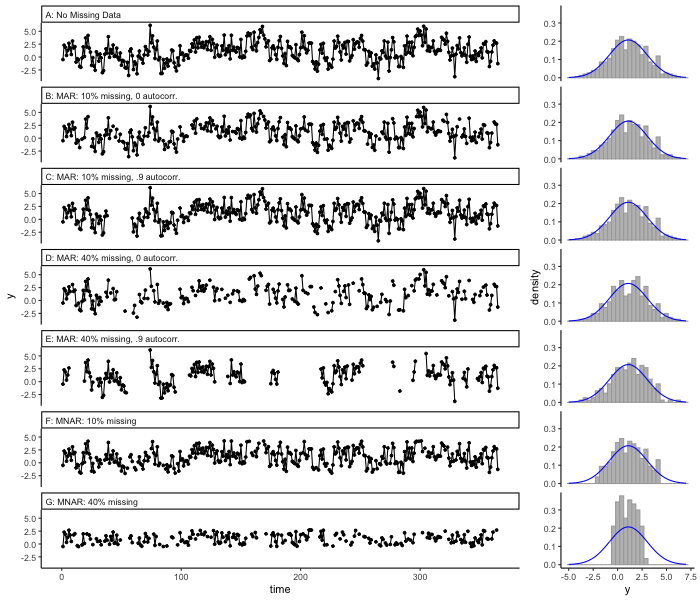
\includegraphics[width = 0.85\textwidth]{Figures/CompareMissingnessTypes_fig.png}
     \caption{An example time series demonstrating different types and amounts of missing data. The left column shows the same time series with different amounts and types of missingness and right column shows the distribution of data points in each resultant time series. A. Complete time series with no missing data. Rows B through E show the time series with 10\% (B and C) or 40\% (D and E) of data missing completely at random (MCAR), with either low autocorrelation in missing data (B and D) or high autocorrelation (C and E). Rows F and G show the time series with data missing not at random (MNAR) for 10\% missing data (F) and 40\% missing data (G).}
     \label{fig:missingtypes}
 \end{figure}

 \begin{figure}
     \noindent\includegraphics[width = 0.85\textwidth]{Figures/MockedUpFigures/heatmap_GaussianMCAR_all.png}
     \caption{Median error of parameter recovery, median absolute error, and model coverage of $\phi$ and $\beta$, depending on the proportion of missing data and autocorrelation in missingness for each of five missing data approaches, using simulated, real-valued datasets with data missing completely at random (MCAR).}
     \label{fig:GaussianMCARheatmapALL}
 \end{figure}

  \begin{figure}
         \noindent\includegraphics[width = 0.85\textwidth]{Figures/MockedUpFigures/heatmap_PoissonMCAR_all.png}
     \caption{Median error of parameter recovery, median absolute error, and model coverage of $\alpha$ and $r$, depending on the proportion of missing data and autocorrelation in missingness for each of five missing data approaches, using simulated time series of counts with data missing completely at random (MCAR). Note that coverage is not shown for the Expectation Maximization approach, since most implementations of this method do not include estimates of standard error.}
     \label{fig:PoissonMCARheatmapALL}
 \end{figure}
 
%\subsection{Bias due to endogeneity}

%It is well known that the ordinary least squares estimator (OLS) of the autoregressive coefficients in an AR($p$) model is biased. To see this, consider a simple AR(1) model with mean zero and variance of the innovations $\sigma^2$. The model can be written as
%$$
%y_t = \phi y_{t-1} + \epsilon_t
%$$
%where $\epsilon_0, ..., \epsilon_n \overset{iid}{\sim} \mathcal{N}(0, \sigma^2)$ and $\phi$ is the autoregressive coefficient. The OLS estimator of $\phi$, $\hat{\phi}$ is obtained by regressing observations $y_1,...,y_n$ against $y_0,...,y_{n-1}$. Thus, the OLS estimator can be written as
%\begin{equation*}
%    \begin{aligned}
%        \hat{\phi} &= \frac{\sum_{t=1}^n y_t y_{t-1}}{\sum_{t=1}^n y_{t-1}^2}\\
%        &= \frac{\sum_{t=1}^n (\phi y_{t-1} + \epsilon_t) y_{t-1}}{\sum_{t=1}^n y_{t-1}^2}\\
%        &= \frac{\sum_{t=1}^n (\phi y_{t-1}^2 + \epsilon_t y_{t-1})}{\sum_{t=1}^n y_{t-1}^2} \\
%        &= \phi \frac{\sum_{t=1}^n y_{t-1}^2}{\sum_{t=1}^n y_{t-1}^2} + \sum_{t=1}^n \frac{y_{t-1}}{\sum_{t=1}^n y_{t-1}^2} \epsilon_t\\
%        &= \phi + \sum_{t=1}^n \frac{y_{t-1}}{\sum_{t=1}^n y_{t-1}^2} \epsilon_t.
%    \end{aligned}
%\end{equation*}
%Taking the expectation,
%\begin{equation*}
%    \mathbb{E}(\hat \phi) = \phi + \mathbb{E}\left(\sum_{t=1}^n \frac{y_{t-1}}{\sum_{t=1}^n y_{t-1}^2} \epsilon_t \right)
%\end{equation*}
%we see that, because the sum in the denominator of the second term in the expectation, $\sum_{t=1}^n y_{t-1}^2$, is not independent of $\epsilon_t$ (if $\epsilon_t$ is large and positive, the sum in the denominator will also increase), the ``covariate" we use is \textit{endogenous}, meaning it is not independent of the errors. The negative correlation between $\epsilon_t$ and the reciprocal of sum $\sum_{t=1}^n y_{t-1}^2$ results in a downward-biased estimator of $\phi$ (i.e, closer to zero). 




\newpage


\end{document}

%%%%%%%%%%%%%%%%%%%%%%%%%%%%%%%
\end{document}
%%%%%%%%%%%%%%%%%%%%%%%%%%%%%%%
